
\documentclass[9pt,twocolumn,twoside]{osajnl}
						
\usepackage{bbm}

\journal{josab} % Choose journal (ao, ol, josaa, josab)

\setboolean{shortarticle}{false} % true = letter, false = research article

\title{Optical trimer, \\ A theoretical physics approach to waveguide couplers}

\author[1]{A. Stoffel}
\author[1,*]{B. M. Rodríguez-Lara}

\affil[1]{Instituto Nacional de Astrof\'{\i}sica, \'Optica y Electr\'onica, Calle Luis Enrique Erro No. 1, Sta. Ma. Tonantzintla, Pue. CP 72840, M\'exico}

\affil[*]{Corresponding author: bmlara@inaoep.mx}

\dates{Compiled \today}

\ociscodes{(050.5298) Photonic crystals; (230.4555) Coupled Resonators; (230.7370) Waveguides;  (350.5500) Propagation.}

\doi{\url{http://dx.doi.org/10.1364/ao.XX.XXXXXX}}

\begin{abstract}
We study electromagnetic field propagation through an ideal, passive, triangular three-waveguide coupler using a symmetry based approach to take advantage of the underlying $SU(3)$ symmetry.
The planar version of this platform has proven valuable in photonic circuit design providing optical sampling, filtering, modulating, multiplexing, and switching.
We show that a group-theory approach can readily provide a starting point for design optimization of the triangular version.
Our analysis is presented as a practical tutorial on the use of group theory to study photonic lattices for those not familiar with abstract algebra methods.
In particular, we study the equilateral trimer to show the relation of pearl-necklace arrays with the Discrete Fourier Transform due to their cyclic group symmetry, and the isosceles trimer to show its relation with the golden ratio and its ability to provide stable output at a single waveguide.  
For the sake of completeness, we go beyond the standard optical-quantum analogy to show that it is possible to derive coupled-mode equations for intensity-phase, and that it is also possible to calculate envelopes for the propagation of all possible inputs belonging to an energy class, as well as individual input field amplitudes, without the need of point-to-point propagation.
\end{abstract}

\setboolean{displaycopyright}{true}

\begin{document}

\maketitle
\thispagestyle{fancy}
\ifthenelse{\boolean{shortarticle}}{\abscontent}{}

%%%%%%%%%%%%%%%%%%%%%%%%%%%%%%%%%%%%%%%%%%%%%%%%%%%%%%%%%%%%%%%%%%%%%%%%%%%%%%%%%%%%%%%%%%%%%%%%%%%
% Introduction
%%%%%%%%%%%%%%%%%%%%%%%%%%%%%%%%%%%%%%%%%%%%%%%%%%%%%%%%%%%%%%%%%%%%%%%%%%%%%%%%%%%%%%%%%%%%%%%%%%%
\section{Introduction}

The planar three-waveguide coupler \cite{Iwasaki1975p100} has proven a reliable platform for optical devices. 
It has been shown to provide tunable sampling, filtering \cite{Haus1981p2321},  modulation \cite{Donelly1985p18} and power coupling \cite{Charczenko1989p202} in voltage driven systems, as well as power dividers and combiners in passive devices \cite{Donelly1983p417,Donelly1986p610,Donelly1987p401,Kubo1989p1924} that have allowed efficient signal referencing for integrated optical biosensors \cite{Luff1998p583}.

In most of the reported literature, optimization seems the standard approach  favored by the optics community to design waveguide couplers \cite{Su1989p1666,Petrovic2015p139} but, recently, analogies with quantum mechanical systems have provided a complementary approach \cite{PerezLeija2013p012309,PerezLeija2013p022303}. 
This has also impacted the design of planar three-waveguide couplers that, for example,  have provided fast, robust directional beam coupling designed either by standard optimization \cite{Ng1999p475,Schneider2001p129,Narevicius2005p3362} or by quantum analogies \cite{Paspalakis2006p30,Salandrino2009p4524,Tseng2013p2478,RodriguezLara2014p013802}.

Here, our aim is to motivate photonic designers to go beyond the standard analogies between photonic lattices and quantum systems. 
We will try our best to bridge the gap between theoretical physics and optics to show how the underlying symmetries of a photonic lattice can shed light into \textcolor{red}{onto} the design process. 
For this, we will use a general version of the three-waveguide coupler.
In the next section, we will introduce the mode-coupling model and expose its underlying $SU(3)$ symmetry. 
Then, we will construct a propagator for any given physical configuration using a Gilmore-Perelomov coherent state approach \cite{VillanuevaVergara2015p}.
In order to provide practical examples, we will focus on arrays of identical waveguides, which we call optical trimers thereon, with three identical couplings and relate them to the discrete Fourier transform through the cyclic group.
We will also present results for the optical trimer with two identical couplings, and relate them to the golden ratio and devices allowing a single intensity stable output. 
Next, for the sake of completeness, we will show that it is possible to recover the coupled mode theory equations for field intensity and phase if we use the optical-quantum analogy in the classical limit.
We will also show that a classical mechanical analysis of the optical-quantum analogy can predict boundary limits for all possible propagation classes defined by a device, as well as propagation envelopes for individual initial inputs without the need of actual propagation.
Finally, we will present a summary and discuss possible extensions allowed by linear and nonlinear three-waveguide couplers.


%%%%%%%%%%%%%%%%%%%%%%%%%%%%%%%%%%%%%%%%%%%%%%%%%%%%%%%%%%%%%%%%%%%%%%%%%%%%%%%%%%%%%%%%%%%%%%%%%%%
% The model and its formal solution
%%%%%%%%%%%%%%%%%%%%%%%%%%%%%%%%%%%%%%%%%%%%%%%%%%%%%%%%%%%%%%%%%%%%%%%%%%%%%%%%%%%%%%%%%%%%%%%%%%%
\section{Triangular three-waveguide coupler}

Light propagating through an ideal, triangular three-waveguide coupler can be described by coupled mode theory, c.f. \cite{RodriguezLara2015p068014} and references therein,
\begin{eqnarray} \label{eq:CMT}
-i \partial_{z} \left( \begin{array}{c} \mathcal{E}_{0}(z) \\ \mathcal{E}_{1}(z) \\  \mathcal{E}_{2}(z) \end{array} \right) =  \left( \begin{array}{ccc} 
\omega_{0}(z)  & g_{01}(z) & g_{02}(z) \\
g_{01}(z) & \omega_{1}(z) & g_{12}(z) \\
g_{02}(z) & g_{12}(z) & \omega_{2}(z)
\end{array} \right) \left( \begin{array}{c} \mathcal{E}_{0}(z) \\ \mathcal{E}_{1}(z) \\  \mathcal{E}_{2}(z) \end{array} \right).
\end{eqnarray}
Here, the complex field amplitude at the $j$th waveguide is given by $\mathcal{E}_{j}(z)$, the effective refractive index at the $j$th waveguide is $\omega_{j}(z)$, and the effective coupling between the $j$th and $k$th waveguides \textcolor{red}{waveguide} is $g_{jk}(z)$.
These complex field equations can be cast in a Schr\"odinger-like form \cite{RodriguezLara2015p068014},
\begin{eqnarray}
- i \partial_{z} \vert \mathcal{E}(z) \rangle = \hat{H}(z) \vert \mathcal{E}(z) \rangle,\label{eq:SchLike}
\end{eqnarray}
where kets and operators in Dirac notation represent column vectors and square matrices, in that order.
We can normalize the intensity, $\sum_{j} \vert \mathcal{E}_{j}(z) \vert^2 =1$, as we are dealing with an ideal lossless device.
Experimental realization of this model include, but are not limited to, laser inscribed photonic waveguides \cite{Szameit2010p163001} and  multicore optical fibers, Fig. \ref{fig:Fig1}(a), whispering-mode cavities \cite{Peng2014p394}, Fig. \ref{fig:Fig1}(b), or microwave resonators \cite{FrancoVillafane2013p170405}.

\begin{figure}[htbp]
\centering
\fbox{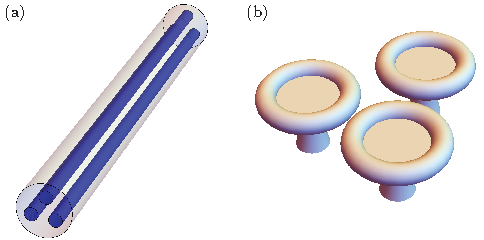
\includegraphics[width=\linewidth]{Fig1.pdf}}
\caption{(Color online) Some experimentally feasible realizations for triangular waveguide couplers, (a)  multicore optical fibers or inscribed photonic waveguides, (b) whispering-gallery mode cavities.}
\label{fig:Fig1}
\end{figure}


The formal solution to this ordinary differential equation,
\begin{eqnarray}
\vert \mathcal{E}(z) \rangle = \hat{U}(z) \vert \mathcal{E}(0) \rangle,
\end{eqnarray}
is provided by an ordered exponential \cite{Magnus1954p649,Blanes2009p151}, 
\begin{eqnarray} 
\hat{U}(z) = \mathrm{Texp} \left[ \int_{0}^{z} \hat{H}(x) dx \right].
\end{eqnarray}
Usually, it is not straightforward to calculate this propagator,
but underlying symmetries simplify this endeavor \cite{Lie1880p441,Wei1963p575,Neumaier2008}.
While group theory is extensively used in mathematical optics \cite{Wolf2004,Lakshminarayanan2012}, it may be possible that the standard Lie algebra approach may look more complicated than it actually is for those outside that field. 
We hope that the following can help vanquish that feeling.


%%%%%%%%%%%%%%%%%%%%%%%%%%%%%%%%%%%%%%%%%%%%%%%%%%%%%%%%%%%%%%%%%%%%%%%%%%%%%%%%%%%%%%%%%%%%%%%%%%%
% How to calculate the propagator and examples
%%%%%%%%%%%%%%%%%%%%%%%%%%%%%%%%%%%%%%%%%%%%%%%%%%%%%%%%%%%%%%%%%%%%%%%%%%%%%%%%%%%%%%%%%%%%%%%%%%%
\section{Group theory approach}

Group theory, as an instrument to explore the underlying structure of mathematical models describing the physical world, brings a layer of abstraction into physics that allows deeper insight.
As such, it has become an essential tool in quantum mechanics.
Coupled mode theory delivers a Schr\"odinger-like form describing light propagating through arrays of coupled waveguides, thus, the use of group theory to calculate propagation in these systems seems like a natural step.

The mode-coupling matrix $\hat{H}$ for our triangular three-waveguide coupler is a unitary matrix of rank three with trace equal to $\sum_{j=0}^{3} \omega_{j}(z)$. 
It is useful to decompose it into a unit matrix part and a traceless part, 
\begin{eqnarray}
	\hat{H}(z) &=& \frac{1}{3} \sum_{j=0}^{3} \omega_{j}(z) \hat{\mathbb{1}} + \hat{\mathcal{H}}(z).
\end{eqnarray}
The traceless part can be written in terms of the special unitary group $SU(3)$ which is  a household name in physics often related to the work of Gell-Mann \cite{GellMann1961} and Ne'eman \cite{Neeman1961p222},
\begin{eqnarray}
	\hat{\mathcal{H}}(z)&=& \frac{1}{2} \omega_{y}(z) \hat{Y}  + \omega_{i}(z) \hat{I}_{0}+ g_{01}(z) \left( \hat{I}_{+} + \hat{I}_{-} \right) \nonumber \\
			&&  + g_{12}(z) \left( \hat{U}_{+} + \hat{U}_{-} \right)  +   g_{02}(z) \left( \hat{V}_{+} + \hat{V}_{-} \right). \label{eq:MCMatrix}
\end{eqnarray}
Here, we have defined the auxiliary effective refractive index $\omega_{y}(z) = \left[ \omega_{0}(z) + \omega_{1}(z) - 2 \omega_{2}(z)\right]/2$, $\omega_{i}(z)= \omega_{0}(z)-\omega_{1}(z)$, and used the following representation for the $SU(3)$ group \cite{Ticciati1999}, 
\begin{eqnarray}
\hat{Y} = \frac{1}{3} \left( \begin{array}{ccc} 
1&0&0\\0&1&0\\0&0&-2    \end{array}\right), \quad
\hat{I}_{0} = \frac{1}{2} \left( \begin{array}{ccc} 1&0&0\\0&-1&0\\0&0&0 \end{array}\right), \quad  
\nonumber\\
\hat{I}_{+} = \left( \begin{array}{ccc} 0&1&0\\0&0&0\\0&0&0 \end{array}\right), \quad 
\hat{I}_{-} = \left( \begin{array}{ccc} 0&0&0\\1&0&0\\0&0&0 \end{array}\right), \quad \nonumber\\
\hat{U}_{+} = \left( \begin{array}{ccc} 0&0&0\\0&0&1\\0&0&0 \end{array}\right), \quad 
\hat{U}_{-} = \left( \begin{array}{ccc} 0&0&0\\0&0&0\\0&1&0 \end{array}\right), \quad \nonumber \\
\hat{V}_{+} = \left( \begin{array}{ccc} 0&0&1\\0&0&0\\0&0&0 \end{array}\right), \quad 
\hat{V}_{-} = \left( \begin{array}{ccc} 0&0&0\\0&0&0\\1&0&0 \end{array}\right), \label{eq:gens}
\end{eqnarray}
due to the fact that we can understand matrices $\hat{I}_{\pm}$, $\hat{U}_{\pm}$ and $\hat{V}_{\pm}$ as those describing the coupling of the electromagnetic field between waveguides zero and one, one and two, and zero and two, in that order, Fig. \ref{fig:Fig2}.

\begin{figure}[htbp]
\centering
\fbox{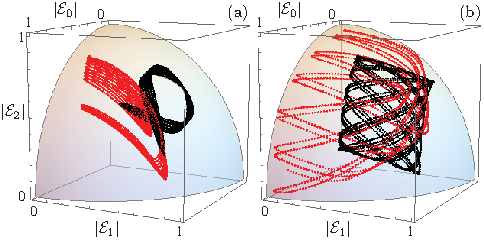
\includegraphics[width=\linewidth]{Fig2.pdf}}
\caption{(Color online) Effective refractive indices and couplings between the waveguides as described by the $SU(3)$ group elements.}
\label{fig:Fig2}
\end{figure}


At this point, our original Schr\"odinger-like equation is written in terms of the identity matrix and a linear combination of Lie group generators for $SU(3)$.
The identity part only induces and overall phase,
\begin{eqnarray}
e^{i \phi(z) \hat{\mathbb{1}}} = e^{\frac{i}{3} \int_{0}^{z} \left(\omega_{0}(\zeta) + \omega_{1}(\zeta) + \omega_{2}(\zeta) \right) d\zeta } ~\hat{\mathbb{1}} .
\end{eqnarray}
such that the propagator can be rewritten,
\begin{eqnarray}
	\hat{U}(z) =  e^{ \frac{i}{3} \int_{0}^{z} ( \omega_{0}(\zeta) + \omega_{1}(\zeta) + \omega_{2}(\zeta) ) d\zeta} ~\hat{\mathcal{U}}(z).
\end{eqnarray}
Now, for the $SU(3)$ part, $\hat{\mathcal{U}}(z)$, Wei and Norman demonstrated that any such equation can be treated by an algebraic method providing the following propagator \cite{Wei1963p575},
\begin{eqnarray}
	\hat{\mathcal{U}}(z) = \prod_{j=1}^{8} e^{i \theta_{j}(z) \hat{X}_{j}},
\end{eqnarray}
where the $su(3)$ algebra elements, $e^{i \theta_{j}(z) \hat{X}_{j}}$, are just the exponential map of the $SU(3)$ group generators, $\left\{ \hat{Y}, \hat{I}_{0}, \hat{I}_{\pm}, \hat{U}_{\pm}, \hat{V}_{\pm} \right\}$, and the functions $\theta_{j}(z)$ are complex functions ruled by the dynamics provided by the mode-coupling matrix, $\hat{\mathcal{H}}(z)$.
There is no apriori ordering of $su(3)$ elements to write the propagator, however, the values of the $\theta_{j}(z)$ functions do depend on the chosen order and different orderings have been studied in the quantum optics literature \cite{Dattoli1987p1582,Dattoli1991p1247,Dattoli1990p236,Gnutzmann1998p9871}.
We will choose a particular ordering,
\begin{eqnarray}
\hat{\mathcal{U}}(z) &=& e^{i \iota_{+}(z) \hat{I}_{+}} e^{i \mu_{+}(z) \hat{U}_{+}}  
e^{i \nu_{+}(z) \hat{V}_{+}} e^{ \iota_{0}(z) \hat{I}_{0}} \nonumber \\ 
&& \times e^{i y_{0}(z) \hat{Y}}  e^{i \nu_{-}(z) \hat{V}_{-}} e^{i \mu_{-}(z) \hat{U}_{-}} e^{i \iota_{-}(z) \hat{I}_{-}}, \label{eq:prop}
\end{eqnarray}
that keeps us in line with the idea of understanding propagation through waveguide lattices as generalized Gilmore-Perelomov coherent states \cite{VillanuevaVergara2015p}.

The next step is straightforward but cumbersome, we substitute the formal solution, $\vert \mathcal{E}(z) \rangle$, using the propagator above and being careful in keeping the ordering through the derivation process. 
Then, we use the actions of elements of the $su(3)$ algebra on elements of the $SU(3)$ group \cite{Nelson1967p857} to find the differential equation set for the auxiliary functions,
\begin{eqnarray}
	\iota_{+}^{\prime} &=&  g_{01} \iota_{+}^{2} +  \left( g_{02} \nu_{+} + i \omega_{i} \right) \iota_{+}  - i g_{12} \nu_{+} + g_{01}    ,    \label{eq:iota} \\
	\mu_{+}^{\prime} &=& \left(g_{12} + i g_{02} \iota_{+} \right)\mu_{+}^{2} + \left[ g_{02} \nu_{+} - g_{01} \iota_{+} + \frac{i}{2} \left(2\omega_{y} - \omega_{i} \right)\right] \mu_{+} \nonumber \\ && + i g_{01} \nu_{+} + g_{12}, \\
	\nu_{+}^{\prime} &=& g_{02} \nu_{+}^{2} +  \left[ g_{01} \iota_{+} + \frac{i}{2} \left( 2 \omega_{y} + \omega_{i}  \right) \right] \nu_{+}  - i g_{12} \iota_{+} + g_{02}  , \label{eq:mu} \\
	\iota_{0}^{\prime} &=& \omega_{i} - i 2  g_{01} \iota_{+} + i g_{12} \mu_{+} - g_{02} \left( \iota_{+} \mu_{+} + i \nu_{+} \right) , \\
	y_{0}^{\prime} &=& \omega_{y} - i\frac{3}{2}  
	[ g_{02}   \nu_{+} +    
	( g_{12} + i  g_{02} \iota_{+})\mu_{+}],  \\
	\nu_{-}^{\prime} &=& g_{02} e^{i  \left( y_0 + \frac{1}{2} \iota_0 \right)}
	 -  e^{i\iota_{0}}   \left( g_{02} \mu_{+} + i  g_{01} \right) \mu_{-} ,  \\
	\mu_{-}^{\prime} &=&  e^{i  \left( y_0 - \frac{1}{2} \iota_0 \right)}
	( g_{12} + i g_{02} \iota_{+}),\\
	\iota_{-}^{\prime} &=& e^{i \iota_{0}} \left( g_{01} - i g_{02}\mu_{+} \right), 
\end{eqnarray}
where, for the sake of space, we have used $f \equiv f(z)$ and $f' \equiv \partial_{z} f(z)$ for auxiliary functions and couplings.


Non-linear differential equations are known to be hard to solve and finding a solution 
often requires intuition and knowledge of the system being analyzed. 
Before delving into details, we would like to point out a key feature of passive, lossless optical models that we are analyzing, their mode-coupling matrices are real symmetric, $\hat{H}^{T}(z) = \hat{H}(z)$ where the operation $O^{T}$ stands for transposition,  and, as a direct consequence, the propagator shares the same property,
\begin{equation}  
	\hat{U}^{T}(z)=\hat{U}(z).
\end{equation} 
This feature allows us to conclude that the propagator functions are symmetric,
\begin{eqnarray}
	\xi_{+}(z)&=&\xi_{-}(z), \quad \xi = \iota, \nu, \mu.
\end{eqnarray}
Furthermore, we observe that two equations, namely Eq.(\ref{eq:iota}) and Eq.(\ref{eq:mu}) only include terms of $\iota_{+}(z)$ and $\nu_{+}(z)$ and their derivatives. 
Therefore, they are decoupled from the rest. 
Most of the time, numerical methods would be the only way to find these auxiliary functions.

An alternate approach can be followed if we write the propagator as a matrix,
\begin{eqnarray}
\hat{\mathcal{U}}(z) = \left( \begin{array}{ccc} 
\Xi(z) & \Sigma(z) & \Theta(z) \\
\Sigma(z) & \Pi(z)    & \Delta(z) \\
\Theta(z) & \Delta(z) & \Gamma(z)
\end{array}  \right),
\end{eqnarray}
where, for reasons that will become apparent in a moment, we introduced a set of five auxiliary functions,
\begin{eqnarray}
	\Gamma(z) &=& e^{- i \frac{2}{3}  y_{0}(z)}, \\
	\Delta(z)&=& i \Gamma(z) \mu_{+}(z), \\
	\Theta(z)&=& \Gamma(z) \left[ -\iota_{+}(z) \mu_{+}(z) + i \nu_{+}(z) \right], \\
	\Pi(z)&=& \Gamma(z) \left[ e^{i y_0 (z)}e^{-i \frac{1}{2}\iota_0 (z)}
		-\mu_{+} (z)^2 \right], \\	
	\Sigma(z)&=& i \iota_{+}(z) \Pi(z) - \Gamma(z) \mu_{+} (z) \nu_{+}(z)), 
\end{eqnarray}
and the sixth can be written in terms of all others,  
\begin{eqnarray}
\Xi(z) = \frac{1 + \Pi(z) \Theta^{2}(z) + \Gamma(z) \Sigma^{2}(z)- 2 \Delta(z) \Theta(z) \Sigma(z)}{ \Pi(z) \Gamma(z) - \Delta^{2}(z)}.
\end{eqnarray}
The original functions can be put in terms of these auxiliary,
\begin{eqnarray}
\iota_{+}(z) &=& i \frac{\Gamma(z)\Sigma(z) - \Delta(z)\Theta(z)}{\Delta^2(z)-\Gamma(z)\Pi(z)}, \\
\mu_{+}(z) &=& -i \frac{\Delta(z)}{\Gamma(z)},\\
\nu_{+}(z) &=& i \frac{\Pi(z)\Theta(z) - \Delta(z)\Sigma(z)}{\Delta^2(z)-\Gamma(z)\Pi(z)} ,\\
\iota_{0}(z) &=& i 2 \log \frac{\Gamma(z) \Pi(z) - \Delta^{2}(z)}{\Gamma^{\frac{1}{2}}(z) } , \\
y_{0}(z) &=& i \frac{3}{2} \log \Gamma(z) .
\end{eqnarray}
Note that the phase functions $y_0(z)$ and $i_0(z)$ are of logarithmic nature and the rest are quotients of the products of the solution basis. 
We now have the simplest matrix differential equation for the propagator \cite{Reid1939p414,Levin1959p519}, 
\begin{eqnarray}
\partial_{z} \hat{\mathcal{U}}(z) = i \mathcal{H} \hat{\mathcal{U}}(z) ,
\end{eqnarray}
with the initial condition $\hat{\mathcal{U}}(0) = \mathbbm{1}$, that translates into,
\begin{eqnarray}
\Theta(z)= 0 , \quad \Delta(z) =  0, \quad \Sigma(z)= 0, \quad
\Gamma(z)= 1, \quad \Pi(z)= 1. \label{eq:initsb}
\end{eqnarray}
This differential equation system is overdetermined due to the characteristics of the original matrix and provides the following identities,
\begin{eqnarray}
g_{01} \left( \Pi - \Xi \right) + g_{02} \Delta - g_{12} \Theta + \omega_{i} \Sigma &=& 0, \\
g_{01} \Delta + g_{02} \left( \Gamma - \Xi \right) - g_{12} \Sigma + \left(  \omega_{y} +\frac{1}{2}\omega_{i}   \right) \Theta &=& 0, \\
g_{01} \Theta - g_{02} \Sigma(z) + g_{12} \left( \Gamma - \Pi \right)  + \left(  \omega_{y} - \frac{1}{2}\omega_{i}\right) \Delta &=& 0. 
\end{eqnarray}
Again, for waveguide couplers that depend on the propagation distance, this formal solution will be analytically tractable only for a handful of cases, for example the planar three-waveguide coupler \cite{RodriguezLara2014p013802}, but it will be always amenable to solution by numerical methods. 

%%%%%%%%%%%%%%%%%%%%%%%%%%%%%%%%%%%%%%%%%%%%%%%%%%%%%%%%%%%%%%%%%%%%%%%%%%%%%%%%%%%%%%%%%%%%%%%%%%
% Case of constant couplings
%%%%%%%%%%%%%%%%%%%%%%%%%%%%%%%%%%%%%%%%%%%%%%%%%%%%%%%%%%%%%%%%%%%%%%%%%%%%%%%%%%%%%%%%%%%%%%%%%%%
\subsection{Optical trimer}
While we have provided a formal solution to propagation through the most general triangular waveguide coupler, considering a particular solution may help build further intuition. 
For the sake of simplicity, let us now consider the constant optical trimer, which is a triangular three-waveguide array with constant couplings and identical waveguides. 
We will introduce the dimensionless propagation parameter $\zeta = g_{01} z$, such that the mode-coupling differential equation becomes 
\begin{eqnarray}
- i \partial_{\zeta} \vert \mathcal{E}(\zeta) \rangle = \hat{\mathcal{H}} \vert \mathcal{E}(\zeta) \rangle, 
\end{eqnarray}
with the mode-coupling matrix,
\begin{eqnarray}
\hat{\mathcal{H}} = \left( \begin{array}{ccc} 
0  & 1 & \alpha  \\
1 & 0 & \beta \\
\alpha & \beta & 0
\end{array} \right), \label{eq:hmlt2}
\end{eqnarray}
given in terms of the dimensionless parameters,
\begin{eqnarray}
\alpha =\frac{g_{02}}{g_{01}}, \quad \beta=\frac{g_{12}}{g_{01}}.
\end{eqnarray}
Now, we can use the results above to build a particular solution, but it is well known that a set of linear first order differential equations is equivalent to a single linear differential equation of higher order.
After some algebra, we can derive a third order differential equation for $\Delta(\zeta)$,
\begin{equation}
\Delta^{\prime\prime\prime}(\zeta) + i(1+\alpha^2+\beta^2)\Delta ^{\prime}(\zeta) -2 \alpha\beta\Delta(\zeta) = 0,\label{eq:ddiff}
\end{equation}
with boundary conditions, 
\begin{eqnarray}
\Delta(0) = 0, \quad \Delta^{\prime}(0) = i\beta, \quad \Delta^{\prime\prime}(0) = -\alpha.
\end{eqnarray}
Note that the remaining auxiliary functions are straightforward to calculate, 
\begin{eqnarray}
\Theta(\zeta)&=& \frac{\beta(1+\beta^2)\Delta(\zeta) - i \alpha\Delta^{\prime}(\zeta)+\beta\Delta^{\prime\prime}(\zeta)}
	{\alpha(1-\beta^2)}  \\
\Gamma(\zeta)&=& \frac{-(1+\beta^2)\Delta(\zeta) +i \alpha\beta\Delta^{\prime}(\zeta)-\Delta^{\prime\prime}(\zeta)}
	{\alpha(1-\beta^2)} \\
\Sigma(\zeta)&=& \frac{\beta(\alpha^2+\beta^2)\Delta(\zeta) -i \alpha\Delta^{\prime}(\zeta)+\beta\Delta^{\prime\prime}(\zeta)}
	{\alpha^2-\beta^2}  \\
\Pi(\zeta)&=& \frac{-\alpha(\alpha^2+\beta^2)\Delta(\zeta) +i \beta\Delta^{\prime}(\zeta)-\alpha\Delta^{\prime\prime}(\zeta)}
	{\alpha^2-\beta^2}.
\end{eqnarray} 

The main auxiliary function $\Delta(\zeta)$ has the following solution,
\begin{eqnarray}
\Delta(\zeta) = \delta_{1} \: e^{i \gamma_1 \zeta} + \delta_{2} \: e^{i \gamma_2 \zeta} +  \delta_{3} \: e^{i \gamma_3 \zeta},
\end{eqnarray}  
where the constant parameters  $\gamma_{j}$ are the eigenvalues of the mode-coupling matrix determined by the characteristic polynomial, a reduced cubic,
\begin{eqnarray}
\gamma_{j}^{3} - (1+ \alpha^{2} + \beta^{2}) \gamma_{j} - 2 \alpha \beta = 0. \label{eq:poly}
\end{eqnarray}
It is straightforward to notice that there are three different real eigenvalues for real, positive, non-zero coupling parameters, $\alpha, \beta > 0$.
These proper values can be writen in a closed but non-compact form, so we will not write them explicitly.
Furthermore, the coefficients are given by
\begin{eqnarray}
\delta_{1} &=& \frac{\alpha-\beta(\gamma_2+\gamma_3)}{(\gamma_1-\gamma_2)(\gamma_1-\gamma_3)},\\
\delta_{2} &=& \frac{\alpha-\beta(\gamma_1+\gamma_3)}{(\gamma_2-\gamma_1)(\gamma_2-\gamma_3)},\\
\delta_{3} &=& \frac{\alpha-\beta(\gamma_1+\gamma_2)}{(\gamma_3-\gamma_1)(\gamma_3-\gamma_2)}. 
\end{eqnarray}  
Thus, the propagator functions, $\iota_{\pm}(z)$, $\mu_{\pm}(z)$, $\nu_{\pm}(z)$, $\iota_{0}(z)$ and $y_{0}(z)$, will effectively contain terms involving the three eigenvalues as well as sums and differences thereof.
Figure \ref{fig: Fig3} shows the trajectories described by the absolute value of the field amplitudes, $\vert \mathcal{E}_{j}(z)\vert$, as they propagate through the constant optical trimer with random parameters and initial field distribution calculated provided by the group theory approach.

\begin{figure}[htbp]
\centering
\fbox{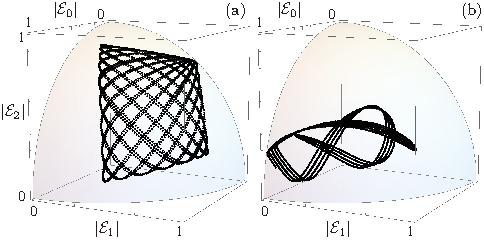
\includegraphics[width=\linewidth]{Fig3.pdf}}
\caption{(Color online) Propagation trajectories of absolute amplitudes, $(\vert \mathcal{E}_{0}(z) \vert, \vert \mathcal{E}_{1}(z) \vert, \vert \mathcal{E}_{2}(z) \vert )$, for two constant optical trimers with random parameters and random normalized initial field distributions.}
\label{fig: Fig3}
\end{figure}



%%%%%%%%%%%%%%%%%%%%%%%%%%%%%%%%%%%%%%%%%%%%%%%%%%%%%%%%%%%%%%%%%%%%%%%%%%%%%%%%%%%%%%%%%%%%%%%%%%%
% Practical examples
%%%%%%%%%%%%%%%%%%%%%%%%%%%%%%%%%%%%%%%%%%%%%%%%%%%%%%%%%%%%%%%%%%%%%%%%%%%%%%%%%%%%%%%%%%%%%%%%%%%

\section{Applications}

As we just saw, the optical trimer is simple enough to allow us the construction of a closed form solution and, to our advantage, it is experimentally feasible to realize it.
Now the obvious question is if there is a use for it.
In the following, we will show that a judicious choice of coupling parameters provides  different types of well-defined propagation of field amplitudes that can be used for the design of integrated photonic circuits.


\subsection{Identical couplings and the discrete Fourier transform}

The mode-coupling matrix for three-identical waveguides distributed in an equilateral triangle configuration, $\alpha = \beta = 1$, 
\begin{equation}
\hat{\mathcal{H}}=\left( \begin{array}{ccc}
0 & 1 & 1 \\
1 & 0 & 1 \\
1 & 1 & 0 \end{array} \right),	 
\end{equation}
is related to the cyclic group in dimension three, 
\begin{eqnarray}
\hat{\mathcal{H}} =  \hat{Z}_{3} + \hat{Z}_{3}^{2} ,
\end{eqnarray}
where the generator of the cyclic group are the following, 
\begin{eqnarray}
\hat{Z}_{3} &=& \hat{I}_{+} + \hat{U}_{+} + \hat{V}_{-}, \nonumber \\
&=&\left(
\begin{array}{ccc}
 0 & 1 & 0 \\
 0 & 0 & 1 \\
 1 & 0 & 0 \\
\end{array}\right).
\end{eqnarray}
It is well known that the cyclic group is diagonalized, 
\begin{eqnarray}
\hat{\Lambda} = \hat{F}_{n} \hat{Z}_{n} \hat{F}_{n}^{\dagger},
\end{eqnarray}
by the discrete Fourier transform of rank $n$ given, for $n=3$,
\begin{eqnarray}
\hat{F}_{3} &=& 
\frac{1}{\sqrt{3}}
\left(
\begin{array}{ccc}
 1 & 1 & 1 \\
 1 & e^{\frac{2 i \pi}{3}} & e^{-\frac{2 i \pi}{3}} \\
 1 & e^{-\frac{2 i \pi}{3}} & e^{\frac{2 i \pi}{3}} \\
\end{array}\right),
\end{eqnarray}
and $\hat{\Lambda}$ is a diagonal rank $n$ matrix showing the $n$th-roots of the unit,
\begin{eqnarray}
\hat{\Lambda}_{mn} = \delta_{m,n} e^{ i \frac{2 \pi}{n} i}, \quad  m,n = 0,1,2,
\end{eqnarray} 
on the main diagonal.
In this particular case, it is possible to compose a propagator,
\begin{eqnarray}
U(\zeta) &=& \hat{F}_{3}^{\dagger} e^{i \hat{\Lambda}_{3} \zeta} e^{i \hat{\Lambda}_{3}^{2} \zeta} \hat{F}_{3}, \nonumber \\
&=& \frac{1}{3}\left(
\begin{array}{ccc}
 2+e^{3 i \zeta} & -1+e^{3 i \zeta} & -1+e^{3 i \zeta} \\
 -1+e^{3 i \zeta} & 2+e^{3 i \zeta} & -1+e^{3 i \zeta} \\
 -1+e^{3 i \zeta} & -1+e^{3 i \zeta} & 2+e^{3 i \zeta} \\
\end{array}
\right) e^{-i \zeta},
\end{eqnarray}
where we have used the fact that the elements of the cyclic group of rank $3$ commute between them, $\left[ \hat{Z}_{3} , \hat{Z}_{3}^{2} \right] = 0$ because $\hat{Z}_{3}^{3} = \mathbb{1}_{3}$.  

Figure \ref{fig: Fig4} shows the trajectories described by the absolute value of the field amplitudes, $\vert \mathcal{E}_{j}(z)\vert$, as they propagate. 
\textcolor{red}{All trajectories will lie on...}
All of trajectories will lie over the surface of an octant of the sphere due to unitary propagation, $\sum_{j} \vert \mathcal{E}_{j}(z) \vert^2 =1$.
Figure \ref{fig: Fig4}(a) shows the response to impulse input, $ \mathcal{E}_{k}(0)  = \delta_{j,k}$ with $j=0,1,2$ and a fixed $k=0,1,2$. 
Figure \ref{fig: Fig3}(b) shows the trajectories given by initial field superpositions of the more general form: $\mathcal{E}_{j} = \alpha_{j} e^{i \phi t}$ with $\alpha \in \mathbb{R}$ and $\sum_{j} \vert \alpha_{j} \vert^{2} =1$.
Note that the roots of the mode-coupling matrix, $\hat{\mathcal{H}}$, are doubly degenerate and commesurate, 
\begin{eqnarray}
\gamma_{1,2} = -1, \quad \gamma_{2\textcolor{red}{3}} = 2.
\end{eqnarray}
Thus, propagation involves just two commensurate eigenvalues and all the possible field amplitude propagation trajectories, $\left( \vert \mathcal{E}_{0} \vert, \vert \mathcal{E}_{1} \vert, \vert \mathcal{E}_{2} \vert  \right)$, will be closed and well defined as those shown in Fig.\ref{fig: Fig3}.


\begin{figure}[htbp]
\centering
\fbox{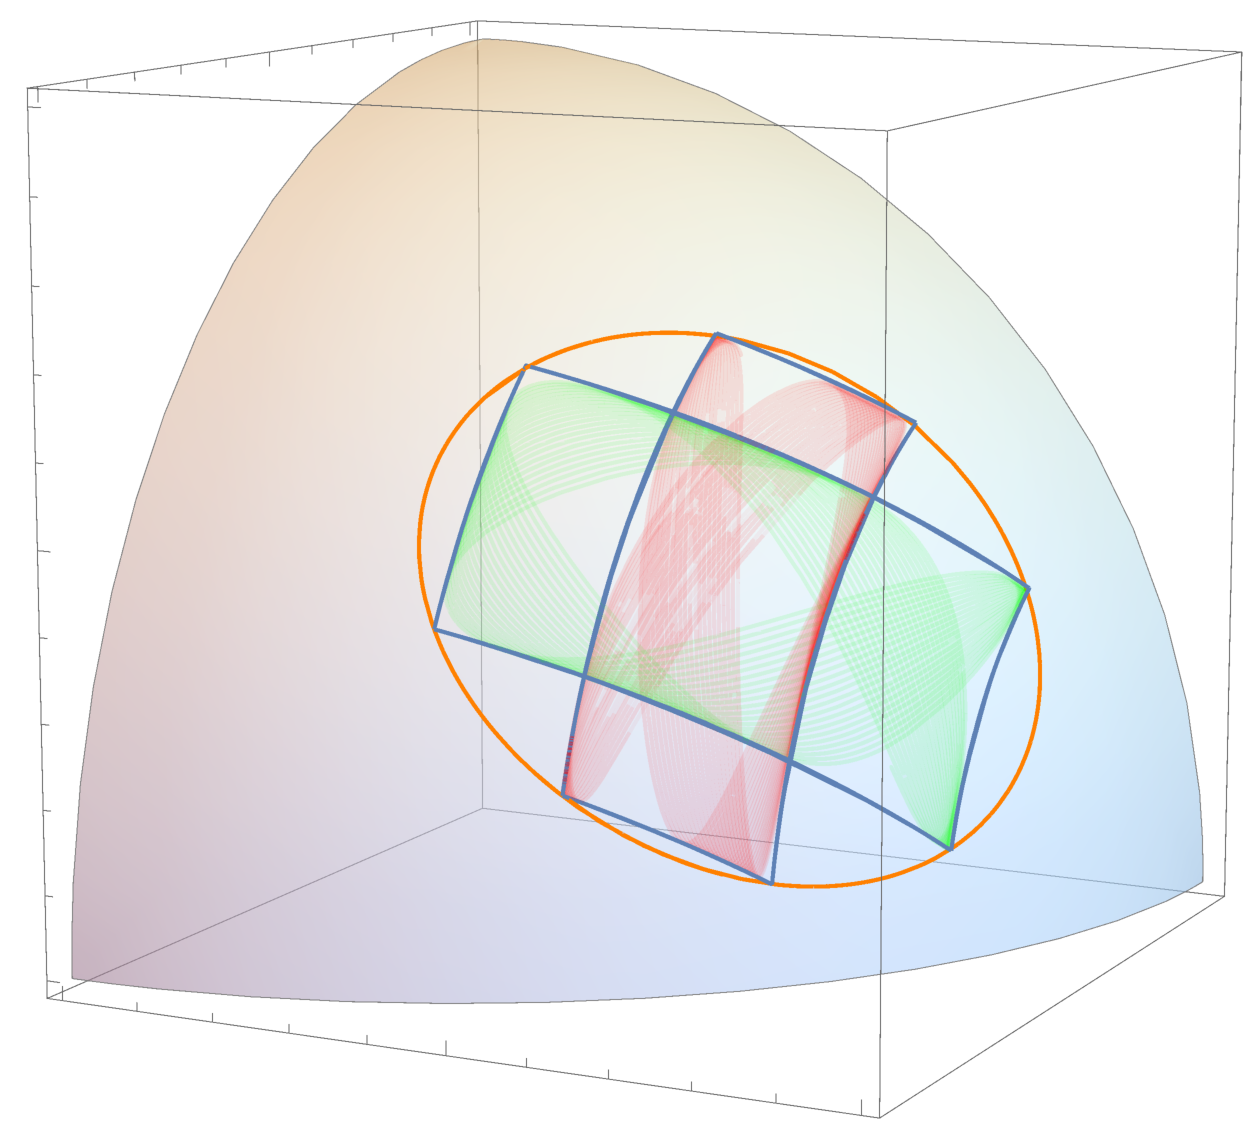
\includegraphics[width=\linewidth]{Fig4.pdf}}
\caption{(Color online) Propagation trajectories of absolute amplitudes, $(\vert \mathcal{E}_{0}(z) \vert, \vert \mathcal{E}_{1}(z) \vert, \vert \mathcal{E}_{2}(z) \vert )$, for initial fields impinging (a) only the zeroth (solid black), $(1,0,0)$, first (dashed blue), $(0,1,0)$, and second (dotted red), $(0,0,1)$, waveguides and (b) initial fields impinging two waveguides at a time with and without a relative phase, $(1,1,0)/ \sqrt{2}$ (solid black), $(1,i,0)/\sqrt{2}$ (dashed blue), and $(2,0,i)/\sqrt{5}$ (dotted red).}
\label{fig: Fig4}
\end{figure}


\subsection{Two identical couplings and the golden ratio}
In the case of two equal coupling parameters the unitless mode-coupling matrix becomes,
\begin{equation}
\hat{\mathcal{H}}=\left( \begin{array}{ccc}
0 & 1 & \alpha \\
1 & 0 & \alpha \\
\alpha & \alpha & 0 \end{array} \right)	 
\end{equation}
Note that exchanging the first and second waveguides returns the same mode-coupling matrix; in other words, it is $\hat{Z}_2$-invariant. 
This symmetry is reflected by the eigenvalues,
\begin{eqnarray}
\gamma_{1} = -1, \quad \gamma_{2} = \bar{\varphi}, \quad \gamma_{3} = \varphi,
\end{eqnarray}  
with
\begin{eqnarray}
\bar{\varphi} &=& \frac{1}{2} \left(1-\sqrt{8 \alpha ^2+1}\right),\\
\varphi &=& \frac{1}{2} \left( 1 + \sqrt{8 \alpha ^2+1} \right).
\end{eqnarray}
It is simply to see that $\bar{\varphi} + \varphi = 1$ and that the latter eigenvalue 
becomes the golden ratio for $\alpha = \sqrt{1/2}$.
Again, due to the $\hat{Z}_2$-symmetry, the propagator can be calculated directly using the group theory approach,
\begin{eqnarray}
\Delta(\zeta) &=& \Theta(z), \\
&=& \frac{\alpha}{\varphi - \tilde{\varphi}} \left(  e^{i \zeta \varphi }  -  e^{i \zeta \bar{\varphi} } \right), \\
\Gamma(\zeta) &=& \frac{1}{\varphi - \tilde{\varphi}} \left( \varphi e^{i \zeta \bar{\varphi} } - \bar{\varphi}  e^{i \zeta \varphi } \right), \\
\Sigma(\zeta) &=& \frac{1}{2 \left( \varphi - \tilde{\varphi} \right)} \left( \varphi e^{i \zeta \varphi } - \bar{\varphi} e^{i \zeta \bar{\varphi} } \right) - \frac{1}{2} e^{-i \zeta}, \\
\Pi(\zeta) &=& \Xi(\zeta), \\
&=& \frac{1}{2 \left( \varphi - \tilde{\varphi} \right)} \left( \varphi e^{i \zeta \varphi } - \bar{\varphi} e^{i \zeta \bar{\varphi} } \right) + \frac{1}{2} e^{-i \zeta}.
\end{eqnarray}

Obviously, when the eigenvalues are commensurate, the field amplitude propagation trajectories will be closed and well defined. 
However, this particular symmetry might allow further interesting states.
Note that the auxiliary functions $\Delta(\zeta)$ and $\Gamma(\zeta)$ depend on only two of the three eigenfrequencies, $\varphi$ and $\bar{\varphi}$. 
Furthermore, a little bit of algebra considering an initial state without any field impinging at the zeroth waveguide, $\mathcal{E}_{0}(0)=0$, reveals that propagation in the second waveguide, $\mathcal{E}_{2}(z)$, only depends on those two auxiliary functions, $\Delta(\zeta)$ and $\Gamma(\zeta)$,
\begin{equation}
\mathcal{E}_{2}(\zeta) = \Delta(\zeta)\mathcal{E}_{1}(0)
+\Gamma(\zeta)\mathcal{E}_{2}(0).
\end{equation}
Now, we can hope that choosing a proper input will cancel out one of the two 
eigenvalues that appear in the evolution of the field amplitude at the second waveguide.
That is, if the evolution only depends on a single eigenvalue, it will only change in phase and the field amplitude at the second waveguide will remain immutable. 
This is fulfilled when either 
\begin{eqnarray}
\mathcal{E}_{1}(0)= \frac{\varphi}{\alpha} \mathcal{E}_{2}(0)\quad \mathrm{or} \quad
\mathcal{E}_{1}(0)= \frac{\bar{\varphi}}{\alpha} \mathcal{E}_{2}(0), \label{eq:IsoIniCon}
\end{eqnarray}
are met as initial conditions.
Without loss of generality, we can give the propagated amplitude vector,
\begin{equation} \label{eq:StatAmp}
\vert \mathcal{E}_{x}(\zeta) \rangle = \frac{1}{\sqrt{\mathcal{N}}}\left( \begin{array}{c}
\frac{\varphi}{\alpha} \Sigma(\zeta) + \Delta(\zeta) \\
\frac{\varphi}{\alpha} \Pi(z) + \Delta(\zeta) \\
e^{i\zeta\varphi}
\end{array} \right)	\quad x= \varphi, \bar{\varphi},
\end{equation}
up to a normalization constant $\mathcal{N}$.
Figure \ref{fig:Fig5} shows propagation trajectories for the absolute field amplitudes in an isoceles constant optical trimer with parameter $\alpha = 1 /\sqrt{2}$ chosen to provide the golden ratio, Fig. \ref{fig:Fig5}(a), and  $\alpha = 1/ 2$, Fig. \ref{fig:Fig5}(b), with initial field amplitudes provided by Eq.(\ref{eq:IsoIniCon}) ensuring a stable output at the second waveguide.

\begin{figure}[htbp]
	\centering
	\fbox{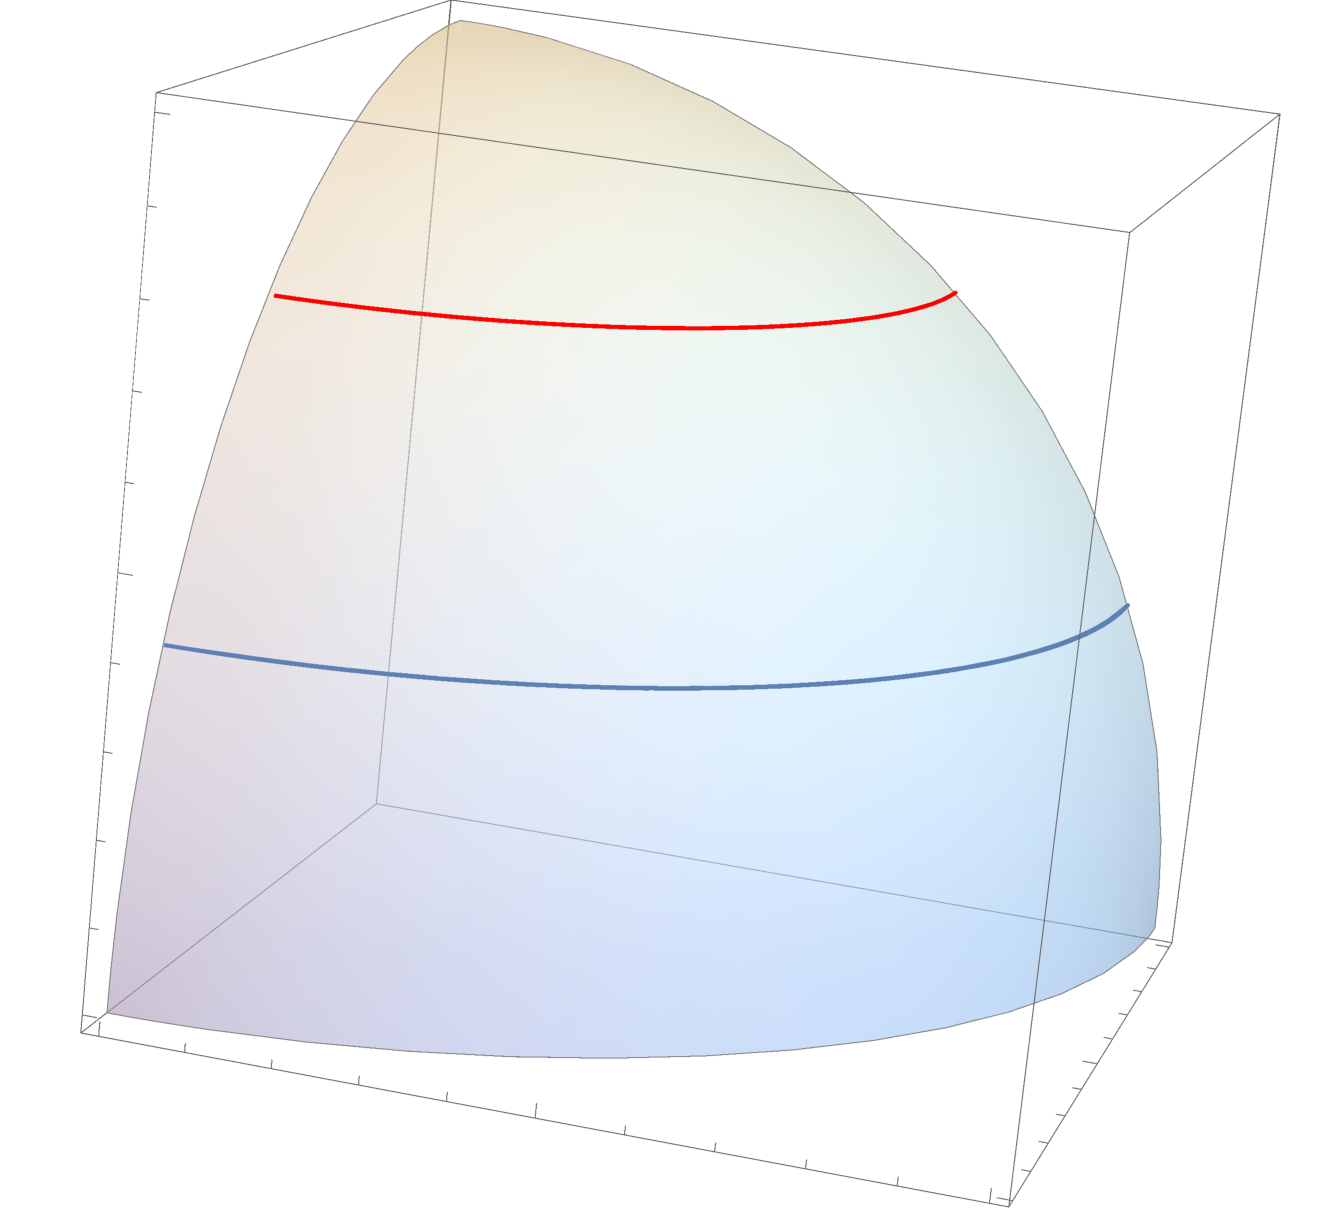
\includegraphics[height=4cm]{Fig5.pdf}}
	\caption{(Color online) Propagation trajectories of absolute amplitudes, $(\vert \mathcal{E}_{0}(z) \vert, \vert \mathcal{E}_{1}(z) \vert, \vert \mathcal{E}_{2}(z) \vert )$,  for the states with stationary field amplitude in the second waveguide related to $\varphi$ (solid black) and $\bar{\varphi}$ (dashed blue) described by Eq.(\ref{eq:StatAmp}) with (a) $\alpha = 1 / \sqrt{2}$ and (b) $\alpha = 1 / 2$ .}
	\label{fig:Fig5}
\end{figure}



%%%%%%%%%%%%%%%%%%%%%%%
%%%% DRAFT
%//////////////////////////////////////////////%//////

\section{Beyond the standard approach}

Finally, we want to show that a theoretical physics treatment of photonic lattices can go beyond the standard approach to the quantum mechanical analogy that considers an array of coupled waveguides as an array of coupled resonators, for the triangular waveguide coupler,
\begin{eqnarray}\label{eq:qmHamiltonian}
	\hat{H}(t) = \sum_{j=0}^{2} \omega_j(t) \hat{a}^{\dagger}_j \hat{a}_{j} + \sum_{j\neq k=0}^{2} g_{jk}(t) \hat{a}^{\dagger}_j \hat{a}_k,
\end{eqnarray}
where the operators $\hat{a}_{j}$ ($\hat{a}_{j}^{\dagger}$) annihilate (create) a photon in the $j$th resonator, and realizes that, with the single photon limit ansatz,
\begin{eqnarray}\label{eq:sglPhoton}
	\left\vert \psi(t) \right\rangle = \mathcal{E}_{0}(t) \left\vert 1, 0, 0 \right\rangle  +
	\mathcal{E}_{1}(t) \left\vert 0,1,0 \right\rangle + \mathcal{E}_{2}(t) \left\vert 0,0,1 \right\rangle,
\end{eqnarray}
with $ \sum_{j} \vert \mathcal{E}_{j}(z) \vert^2 = 1$, it yields the same system of differential equations,
\begin{eqnarray} \label{eq:}
	i \partial_t	
	\left( \begin{array}{c} 
		\mathcal{E}_{0}(t) \\
		\mathcal{E}_{1}(t) \\
		\mathcal{E}_{2}(t)
	\end{array} \right) =
	\left( \begin{array}{ccc} 
		\omega_{0}(t)  & g_{01}(t) & g_{02}(t) \\
		g_{01}(t) & \omega_{1}(t) & g_{12}(t) \\
		g_{02}(t) & g_{12}(t) & \omega_{2}(t)
	\end{array} \right)
	\left( \begin{array}{c} 
		\mathcal{E}_{0}(t) \\
		\mathcal{E}_{1}(t) \\
		\mathcal{E}_{2}(t)
	\end{array} \right),
\end{eqnarray}
than \textcolor{red}{ as }coupled-mode theory, Eq.(\ref{eq:CMT}), once we make the substitution $t=-z$. 
This analogy allowed us to pursuit a group theory approach in the previous sections for the propagation of the field amplitudes but it can also allows \textcolor{red}{allow us??} to go further and derive equations of motion for different sets of variables.

\subsection{Classical limit and intensity-phase equations}
For example, if we forget about the single-photon limit and take the classical limit, where the states of light can be taken as coherent states with a high number of photons, then, the canonical pair provided by the creation and annihilation operators can be replaced by the canonical pair of classical intensity, $n_{j}$, and phase, $\phi_{j}$, such that $\hat{a}_{j} \rightarrow \sqrt{n_{j}} e^{i \phi_{j}}$, we obtain a classical Hamiltonian, 
\begin{eqnarray}\label{eq:clHamiltonian}
	H(z) = \sum_{j=0}^{2} \omega_{j}(z) n_{j}  
	+ \sum_{j \neq k = 0}^{2} g_{jk}(z) \sqrt{n_{j} n_{k}} \cos \left( \phi_{j} - \phi_{k} \right),
\end{eqnarray}
that provides us with the following equations of motion for the classical canonical pairs, 
\begin{eqnarray}
	\partial_z n_j(z) &=& -\frac{\partial H(z)}{\partial \phi_j}\\
	\partial_z \phi_j(z) &=& \frac{\partial H(z)}{\partial n_j},
\end{eqnarray}
where we have already accounted for the switch from time to propagation distance.
These six coupled differential equations for the three degrees of freedom can be reduced to two degrees of freedom if we substitute the intensity $n_{2}(z) = 1 - n_{0}(z)- n_{1}(z)$ and use the phase $\phi_{2}(z)$ as reference, such that we define the phase differences $\delta_{j}(z) = \phi_{j}(z) - \phi_{2}(z)$ for $j=0,1$, ending up with just four coupled differential equations.
This result is the coupled mode theory description of the propagation of intensity and phase.

\subsection{Classical mechanics and propagation envelopes }
We can also choose the standard classical mechanics canonical pair  provided by the field quadratures, 
\begin{eqnarray}
	\hat{q} = \frac{1}{\sqrt{2}} \left( \hat{a}^{\dagger} + \hat{a} \right), ~ 
	\hat{p} = \frac{i}{\sqrt{2}} \left( \hat{a}^{\dagger} + \hat{a} \right),
\end{eqnarray}
and, again, consider classical variables to obtain equations of motion for the field quadratures,
\begin{eqnarray}
	i \partial_z \vert p(z) \rangle	
	 &=&
	H(z) \vert q(z) \rangle , \\
-	i \partial_z \vert q(z) \rangle	 &=& 
    H(z)	\vert p(z) \rangle,
\end{eqnarray}
where, again, we have used kets to represent column vectors, $\vert x(z) \rangle = \left( x_{0}(z), x_{1}(z), x_{2}(z) \right)^{T}$ with $x=p,q$, and made the change from time to propagation distance.
Before moving on, let us focus on the absolute value of the field amplitudes that we have been using to plot the dynamics of our optical trimers, $(\vert \mathcal{E}_{0} \vert,\vert \mathcal{E}_{1} \vert,\vert \mathcal{E}_{2} \vert )$.
These square roots of the intensities at the three waveguides can be understood as a Poincar\'e phase space in the classical mechanics sense.
Then, we can follow a standard classical mechanics approach to find the action-phase variables of the system \cite{Goldstein1980}. 
If the phases are commensurate, the trajectories in phase space will be periodic, and if the phases are incommensurate, the trajectories will be ergodic and fill a region of the phase space defined by the energy of the initial state,
\begin{eqnarray}
\epsilon = \langle \mathcal{E}(0) \vert \hat{H}(0) \vert \mathcal{E}(0) \rangle.
\end{eqnarray}  
For mode-coupling matrices that do not depend on the propagation distance, if the eigenvalues are commensurable, the trajectories in phase space are well-defined and closed, otherwise they will fill a region defined by the initial energy.
Figure \ref{fig:Fig6} shows propagation trajectories of the absolute field amplitudes for the numerical propagation of random parameter sets and initial conditions yielding incommensurate eigenvalues and, thus, ergodic trajectories.

\begin{figure}[htbp]
	\centering
	\fbox{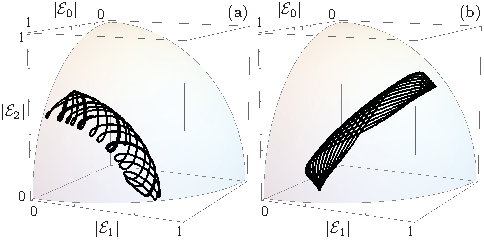
\includegraphics[width=\linewidth]{Fig6.pdf}}
	\caption{(Color online) Propagation trajectories of absolute amplitudes, $(\vert E_{0}(z) \vert, \vert E_{1}(z) \vert, \vert E_{2}(z) \vert )$, for initial random fields impinging random triangular three-waveguide couplers with constant parameters yielding ergodic trajectories.}
	\label{fig:Fig6}
\end{figure}

Let us focus our attention now on the vast class of incommensurate trajectories and, for the sake of simplicity, keep using optical devices that do not change with the propagation distance.
In many design circumstances, the exact point-to-point evolution of the field amplitudes is not of primary importance and it suffices to gain information on the general region that will be traversed. 
This is characterized by the boundary which encompasses the very region. 
It proves viable to notice that for a given energy, $\epsilon$, and a given set of parameters, $\omega_{j}$ and $g_{jk}$, in most cases, an infinity number of distinct trajectories prevails.
The conjunction of all these propagation trajectories pertaining 
\textcolor{red}{to}
a given energy span a path-connected surface.
We will now find the outer boundary, or envelope, of all propagation trajectories related to an initial energy $\epsilon$.
Equation (\ref{eq:clHamiltonian}) readily reveals that the energy is maximized for given intensities $n_0$, $n_1$ and $n_2$ when all three phases are zero. 
Consequently, the boundary is defined by all triplets $\left( n_0,n_1,n_2 \right)$ that fulfill the following condition,
\begin{equation}
	H_{B}(n_0,n_1,n_2) = \epsilon,	
\end{equation}
with 
\begin{eqnarray}
H_{B}(n_0,n_1,n_2) = \sum_{j=0}^{2} \omega_{j} n_{j}  
	+ \sum_{j \neq k = 0}^{2} g_{jk} \sqrt{n_{j} n_{k}}.
\end{eqnarray}
Due to our normalization requirements, $\sum_{j=0}^{2} n_{j} = 1$, the three intensities are not independent and we can safely omit the third intensity in the following discussion,  
$H_{B}(n_0,n_1,n_2) \rightarrow H_{B}(n_0,n_1)$.
Numerically, once a given set of initial intensities or energy is chosen, the envelope is characterized by the following differential equation,
\begin{eqnarray}
	\frac{\partial H_{B}}{\partial n_1}\delta n_1 + 
	\frac{\partial H_{B}}{\partial n_2}\delta n_2 = 0.
\end{eqnarray}
This is the envelope for all possible trajectories with energy $\epsilon$.
Figure \ref{fig:Fig7} shows such envelope as a solid black line.

Now, we can turn to calculate
\textcolor{red}{calculating} the envelope of a single trajectory. 
We have already discussed how to find the propagator for any given three-waveguide coupler. 
In the particular case at hand, constant effective refractive indices and couplings, the propagated field can be written as, 
\begin{eqnarray}
	\vert \mathcal{E}(z) \rangle =  \sum_{j=1}^{3} c_j e^{i \gamma_j z} \vert e_j \rangle,
\end{eqnarray}
where the vectors $\vert e_j \rangle$ are the three normal modes of the coupler with corresponding eigenvalues $\omega_j$ and the normal mode decomposition parameters are defined as the inner product between the normal mode and the initial condition,  $c_{j} = \langle e_{j} \vert \mathcal{E}(0) \rangle$. 
We can introduce a phase relevant parameter which distorts the ratio between eigenvalues, 
\begin{eqnarray}
\vert \mathcal{E}(z, \phi) \rangle = c_0 e^{i \left( \gamma_0 z + \phi \right) } \vert e_0 \rangle + c_1 e^{i \gamma_1 z} \vert e_1 \rangle + c_2 e^{i \gamma_2 z} \vert e_2 \rangle,
\end{eqnarray}
The parameter $\phi$ makes a given trajectory or, more precisely, a section of the trajectory, offset in a direction perpendicular to the trajectory \textcolor{red}{Not sure if the sentence is good}.
This however cannot hold true at the envelope and, hence, we can establish the following condition for the envelope,
\begin{eqnarray}
	\frac{ (\frac{\partial n_0}{\partial z}) }{ (\frac{\partial n_1}{\partial z}) } = \frac{( \frac{\partial n_0}{\partial \phi})}{(\frac{\partial n_1}{\partial \phi}) } ,
\end{eqnarray}
which is identical to requiring a null determinant,
\begin{eqnarray}
	D(z, \phi) &=& \left\vert \left(  \begin{array}{cc} 
		\frac{\partial n_0}{\partial z} & \frac{\partial n_1}{\partial z} \\
		\frac{\partial n_0}{\partial \phi} & \frac{\partial n_1}{\partial \phi} 
	\end{array} \right) \right\vert, \\
	&=& 0.
\end{eqnarray}
Accordingly, the envelope can be calculated from the following differential equation,
\begin{eqnarray}
	\frac{\partial D(z,\phi)}{\partial z} \delta z +
	\frac{\partial D(z,\phi)}{\partial \phi} \delta \phi = 0. \label{eq:EnvInd}
\end{eqnarray}
Figure \ref{fig:Fig7} shows two examples of envelopes of individual trajectories with particular initial field amplitudes as dashed blue and dotted red lines. 

\begin{figure}[htbp]
	\centering
	\fbox{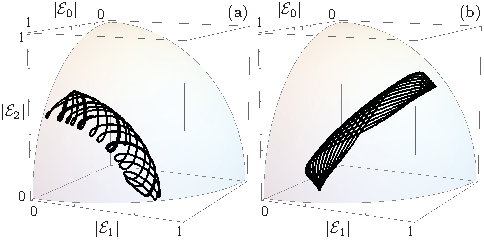
\includegraphics[height=4cm]{Fig7.pdf}}
	\caption{(Color online) Propagation trajectories of absolute amplitudes, $(\vert E_{0}(z) \vert, \vert E_{1}(z) \vert, \vert E_{2}(z) \vert )$,  for two 
		distinct trajectories pertaining to the energy $\epsilon$ (solid gray). The boundary of all possible trajectories (solid black) and the envelopes of the individual  trajectories (dashed blue and dotted red) are calculated according to equation Eq.(\ref{eq:EnvInd}).} 
	
	\label{fig:Fig7}
\end{figure}


\section{Conclusion}
We have shown that it is possible to approach the propagation of electromagnetic field through triangular three-waveguide couplers, in terms of the Lie algebra $su(3)$. 
We derived a formal solution \`a la Wei-Norman in line with the idea of Gilmore-Perelomov coherent states.
In order to provide practical examples, we focused our attention on a reduced class of structures where the waveguides are identical and the effective couplings are constant, independent of the propagation distance, and called \textcolor{red}{coined them??} these systems constant optical trimers. 
We established a connection between the equilateral trimer, actually any circular array of waveguides with identical couplings, and the discrete Fourier transform, and between the isoceles trimer and the golden ratio where it is possible to suppress the energy transfer to one of the waveguides. 

We went beyond the standard classical-quantum analogy in the single photon limit and showed that, using the classical limit, it is possible to recover the coupled mode differential equations describing the propagation of intensity and phase.
Furthermore, we also showed that choosing to work with the classical mechanics canonical pair, which are the equivalent of the electromagnetic field quadratures, allows us to calculate the envelope of all possible trajectories with a given initial energy as well as individual envelopes for specific input field amplitude distributions.
All these results may provide a working platform for the design of photonic integrated devices where the main interest is to generate a specific output from a set of particular inputs instead of studying point-to-point propagation through the devices.

We hope this manuscript could also serve as a tutorial for the use of theoretical physics tools in the design of photonic lattices and, viceversa, encourage theoretical physicists to make incursions on the field of photonic circuit design.



%\section*{Funding Information}

%\textbf{Funding.} 

%\section*{Acknowledgments}

%\textbf{Acknowledgment.} 


%\section*{References}
% Bibliography
\bibliographystyle{osajnl}
\bibliography{D:/ExternalHD/Bibliography/references}


\end{document}

=======
\documentclass[9pt,twocolumn,twoside]{osajnl}
						
\usepackage{bbm}

\journal{josaa} % Choose journal (ao, ol, josaa, josab)

\setboolean{shortarticle}{false} % true = letter, false = research article

\title{Optical trimer, \\ A theoretical physics approach to waveguide couplers}

\author[1]{A. Stoffel}
\author[1,*]{B. M. Rodríguez-Lara}

\affil[1]{Instituto Nacional de Astrof\'{\i}sica, \'Optica y Electr\'onica, Calle Luis Enrique Erro No. 1, Sta. Ma. Tonantzintla, Pue. CP 72840, M\'exico}

\affil[*]{Corresponding author: bmlara@inaoep.mx}

\dates{Compiled \today}

\ociscodes{(050.5298) Photonic crystals; (230.4555) Coupled Resonators; (230.7370) Waveguides;  (350.5500) Propagation.}

\doi{\url{http://dx.doi.org/10.1364/ao.XX.XXXXXX}}

\begin{abstract}
We study electromagnetic field propagation through an ideal, passive, triangular three-waveguide coupler using a symmetry based approach to take advantage of the underlying $SU(3)$ symmetry.
The planar version of this platform has proven valuable in photonic circuit design providing optical sampling, filtering, modulating, multiplexing, and switching.
We show that a group-theory approach can readily provide a starting point for design optimization of these devices.
We also try to present our analysis as a practical tutorial on the use of group theory to study photonic lattices for those not familiar with abstract algebra methods.
\end{abstract}

\setboolean{displaycopyright}{true}

\begin{document}

\maketitle
\thispagestyle{fancy}
\ifthenelse{\boolean{shortarticle}}{\abscontent}{}

%%%%%%%%%%%%%%%%%%%%%%%%%%%%%%%%%%%%%%%%%%%%%%%%%%%%%%%%%%%%%%%%%%%%%%%%%%%%%%%%%%%%%%%%%%%%%%%%%%%
% Introduction
%%%%%%%%%%%%%%%%%%%%%%%%%%%%%%%%%%%%%%%%%%%%%%%%%%%%%%%%%%%%%%%%%%%%%%%%%%%%%%%%%%%%%%%%%%%%%%%%%%%
\section{Introduction}

The planar three-waveguide coupler \cite{Iwasaki1975p100} has proven a reliable platform for optical devices. 
It has been shown to provide tunable sampling, filtering \cite{Haus1981p2321},  modulation \cite{Donelly1985p18} and power coupling \cite{Charczenko1989p202} in voltage driven systems, as well as power dividers and combiners in passive devices \cite{Donelly1983p417,Donelly1986p610,Donelly1987p401,Kubo1989p1924} that have allowed efficient signal referencing for integrated optical biosensors \cite{Luff1998p583}.

In most of the reported literature, optimization seems the standard approach  favored by the optics community to design waveguide couplers \cite{Su1989p1666,Petrovic2015p139} but, recently, analogies with quantum mechanical systems have provided an alternative complementary approach \cite{PerezLeija2013p012309,PerezLeija2013p022303}. 
This has also impacted the design of planar three-waveguide couplers that, for example,  have provided fast, robust directional beam coupling designed either by standard optimization \cite{Ng1999p475,Schneider2001p129,Narevicius2005p3362} or by quantum analogies \cite{Paspalakis2006p30,Salandrino2009p4524,Tseng2013p2478,RodriguezLara2014p013802}.

Here, our aim is to motivate photonic designers to go beyond analogies between photonic lattices and quantum systems. 
We will try our best to bridge the gap between theoretical physics and optics to show how the underlying symmetries of a photonic lattice can shed light into the design process. 
For this, we will use a general version of the three-waveguide coupler.
In the next section, we will introduce the mode-coupling model and expose its underlying $SU(3)$ symmetry. 
Then, we will show how to construct a propagator for any given physical configuration using a Gilmore-Perelomov coherent state approach \cite{VillanuevaVergara2015p}.
In order to provide practical examples, we will focus on arrays of identical waveguides with three identical couplings, which are related to the discrete Fourier transform, an two identical couplings, which are related to the golden ratio and allow devices with a single stable output. 
Finally, we will present a summary with possible extensions allowed by linear and nonlinear three-waveguide couplers.


%%%%%%%%%%%%%%%%%%%%%%%%%%%%%%%%%%%%%%%%%%%%%%%%%%%%%%%%%%%%%%%%%%%%%%%%%%%%%%%%%%%%%%%%%%%%%%%%%%%
% The model and its formal solution
%%%%%%%%%%%%%%%%%%%%%%%%%%%%%%%%%%%%%%%%%%%%%%%%%%%%%%%%%%%%%%%%%%%%%%%%%%%%%%%%%%%%%%%%%%%%%%%%%%%
\section{Three-waveguide coupler}

Light propagating through an ideal, general three-waveguide coupler can be described by coupled mode theory, c.f. \cite{RodriguezLara2015p068014} and references therein,
\begin{eqnarray}\label{eq:principal}
-i \partial_{z} \left( \begin{array}{c} \mathcal{E}_{0}(z) \\ \mathcal{E}_{1}(z) \\  \mathcal{E}_{2}(z) \end{array} \right) =  \left( \begin{array}{ccc} 
\omega_{0}(z)  & g_{01}(z) & g_{02}(z) \\
g_{01}(z) & \omega_{1}(z) & g_{12}(z) \\
g_{02}(z) & g_{12}(z) & \omega_{2}(z)
\end{array} \right) \left( \begin{array}{c} \mathcal{E}_{0}(z) \\ \mathcal{E}_{1}(z) \\  \mathcal{E}_{2}(z) \end{array} \right).
\end{eqnarray}
Here, the complex field amplitude at the $j$th waveguide is given by $\mathcal{E}_{j}(z)$, the effective refractive index at the $j$th waveguide is $\omega_{j}(z)$, and the effective coupling between the $j$th and $k$th waveguides is $g_{jk}(z)$.
These complex field equations can be cast in a Schr\"odinger-like form \cite{RodriguezLara2015p068014},
\begin{eqnarray}
- i \partial_{z} \vert \mathcal{E}(z) \rangle = \hat{H}(z) \vert \mathcal{E}(z) \rangle,\label{eq:diff}
\end{eqnarray}
where kets and operators in Dirac notation represent column vectors and square matrices, in that order.
We can normalize the intensity, $\sum_{j} \vert \mathcal{E}_{j}(z) \vert^2 =1$, as we are dealing with an ideal lossless device.
Experimental realization of this model include, but are not limited, to laser inscribed photonic waveguides \cite{Szameit2010p163001} and  multicore optical fibers \cite{}, Fig. \ref{fig:Fig1}(a), whispering-mode cavities \cite{}, Fig. \ref{fig:Fig1}(b), or microwave resonators \cite{FrancoVillafane2013p170405} and, outside the field of optics,  standard RLC-circuits \cite{}.

The formal solution,
\begin{eqnarray}
\vert \mathcal{E}(z) \rangle = \hat{U}(z) \vert \mathcal{E}(0) \rangle,
\end{eqnarray}
to this ordinary matrix linear differential equation is provided by an ordered exponential \cite{Magnus1954p649,Blanes2009p151}, 
\begin{eqnarray} 
\hat{U}(z) = \mathrm{Texp} \left[ \int_{0}^{z} \hat{H}(x) dx \right].
\end{eqnarray}
Usually, it is not straightforward to calculate this propagator,
but underlying symmetries simplify this endeavor \cite{Lie1880p441,Wei1963p575,Neumaier2008}.
While group theory is extensively used in mathematical optics \cite{Wolf2004,Lakshminarayanan2012}, it may be possible that the standard Lie algebra approach may look more complicated than it actually is for those outside that field. 
We hope that the following can help vanquish that feeling.


%%%%%%%%%%%%%%%%%%%%%%%%%%%%%%%%%%%%%%%%%%%%%%%%%%%%%%%%%%%%%%%%%%%%%%%%%%%%%%%%%%%%%%%%%%%%%%%%%%%
% How to calculate the propagator and examples
%%%%%%%%%%%%%%%%%%%%%%%%%%%%%%%%%%%%%%%%%%%%%%%%%%%%%%%%%%%%%%%%%%%%%%%%%%%%%%%%%%%%%%%%%%%%%%%%%%%
\section{Group theory approach}

Group theory, as an instrument to explore the underlying structure of mathematical models describing the physical world, brings a layer of abstraction into physics that allows deeper insight.
As such, it has become an essential tool in quantum mechanics.
Coupled mode theory delivers a Schr\"odinger-like form describing light propagating through arrays of coupled waveguides, thus, the use of group theory to calculate propagation in these systems seems like a natural step.

The mode-coupling matrix $\hat{H}$ for our triangular three-waveguide coupler is a unitary matrix of rank three with trace equal to $\sum_{j=0}^{3} \omega_{j}(z)$. 
It is useful to decomposed it into a unit matrix part and a traceless part, 
\begin{eqnarray}
	\hat{H}(z) &=& \frac{1}{3} \sum_{j=0}^{3} \omega_{j}(z) \hat{\mathbb{1}} + \hat{\mathcal{H}}(z).
\end{eqnarray}
The traceless part can be written in terms of the special unitary group $SU(3)$ which is  a household name in physics often related to the work of Gell-Mann \cite{GellMann1961} and Ne'eman \cite{Neeman1961p222},
\begin{eqnarray}
	\hat{\mathcal{H}}(z)&=& \frac{1}{2} \omega_{y}(z) \hat{Y}  + \omega_{i}(z) \hat{I}_{0}+ g_{01}(z) \left( \hat{I}_{+} + \hat{I}_{-} \right) \nonumber \\
			&&  + g_{12}(z) \left( \hat{U}_{+} + \hat{U}_{-} \right)  +   g_{02}(z) \left( \hat{V}_{+} + \hat{V}_{-} \right). \label{eq:MCMatrix}
\end{eqnarray}
Here, we have defined the auxiliary effective refractive index $\omega_{y}(z) = \left[ \omega_{0}(z) + \omega_{1}(z) - 2 \omega_{2}(z)\right]/2$, $\omega_{i}(z)= \omega_{0}(z)-\omega_{1}(z)$, and used the following representation for the $SU(3)$ group \cite{Ticciati1999}, 
\begin{eqnarray}
\hat{Y} = \frac{1}{3} \left( \begin{array}{ccc} 
1&0&0\\0&1&0\\0&0&-2    \end{array}\right), \quad
\hat{I}_{0} = \frac{1}{2} \left( \begin{array}{ccc} 1&0&0\\0&-1&0\\0&0&0 \end{array}\right), \quad  
\nonumber\\
\hat{I}_{+} = \left( \begin{array}{ccc} 0&1&0\\0&0&0\\0&0&0 \end{array}\right), \quad 
\hat{I}_{-} = \left( \begin{array}{ccc} 0&0&0\\1&0&0\\0&0&0 \end{array}\right), \quad \nonumber\\
\hat{U}_{+} = \left( \begin{array}{ccc} 0&0&0\\0&0&1\\0&0&0 \end{array}\right), \quad 
\hat{U}_{-} = \left( \begin{array}{ccc} 0&0&0\\0&0&0\\0&1&0 \end{array}\right), \quad \nonumber \\
\hat{V}_{+} = \left( \begin{array}{ccc} 0&0&1\\0&0&0\\0&0&0 \end{array}\right), \quad 
\hat{V}_{-} = \left( \begin{array}{ccc} 0&0&0\\0&0&0\\1&0&0 \end{array}\right), \label{eq:gens}
\end{eqnarray}
due to the fact that we can understand matrices $\hat{I}_{\pm}$, $\hat{U}_{\pm}$ and $\hat{V}_{\pm}$ as those describing the coupling of the electromagnetic field between waveguides zero and one, one and two, and zero and two, in that order.

At this point, our original Schr\"odinger-like equation is written in terms of the identity matrix and a linear combination of Lie group generators for $SU(3)$.
The identity part only induces and overall phase,
\begin{eqnarray}
e^{i \phi(z) \hat{\mathbb{1}}} = e^{\frac{i}{3} \int_{0}^{z} \left(\omega_{0}(\zeta) + \omega_{1}(\zeta) + \omega_{2}(\zeta) \right) d\zeta } ~\hat{\mathbb{1}} .
\end{eqnarray}
such that,
\begin{eqnarray}
	\hat{U}(z) =  e^{ \frac{i}{3} \int_{0}^{z} ( \omega_{0}(\zeta) + \omega_{1}(\zeta) + \omega_{2}(\zeta) ) d\zeta} ~\hat{\mathcal{U}}(z).
\end{eqnarray}
Now, for the $SU(3)$ part $\hat{\mathcal{U}}(z)$, Wei and Norman demonstrated that any such equation can be treated by an algebraic method providing the following propagator \cite{Wei1963p575},
\begin{eqnarray}
	\hat{\mathcal{U}}(z) = \prod_{j=1}^{8} e^{i \theta_{j}(z) \hat{X}_{j}},
\end{eqnarray}
where the $su(3)$ algebra elements, $e^{i \theta_{j}(z) \hat{X}_{j}}$, are just the exponential map of the group generators, $\left\{ \hat{Y}, \hat{I}_{0}, \hat{I}_{\pm}, \hat{U}_{\pm}, \hat{V}_{\pm} \right\}$, and the functions $\theta_{j}(z)$ are complex functions ruled by the dynamics provided by the mode-coupling matrix, $\hat{H}$.
Note, there is no apriori ordering of $su(3)$ elements to write the propagator. 
However, the values of the $\theta_{j}(z)$ functions do depend on the chosen order Different orderings have been studied in the quantum optics literature \cite{Dattoli1987p1582,Dattoli1991p1247,Dattoli1990p236,Gnutzmann1998p9871}.
We will choose a particular ordering,
\begin{eqnarray}
\hat{\mathcal{U}}(z) &=& e^{i \iota_{+}(z) \hat{I}_{+}} e^{i \mu_{+}(z) \hat{U}_{+}}  
e^{i \nu_{+}(z) \hat{V}_{+}} e^{ \iota_{0}(z) \hat{I}_{0}} \nonumber \\ 
&& \times e^{i y_{0}(z) \hat{Y}}  e^{i \nu_{-}(z) \hat{V}_{-}} e^{i \mu_{-}(z) \hat{U}_{-}} e^{i \iota_{-}(z) \hat{I}_{-}}, \label{eq:prop}
\end{eqnarray}
that keeps us in line with the idea of understanding propagation through waveguide lattices as generalized Gilmore-Perelomov coherent states \cite{VillanuevaVergara2015p}.

The next step is straightforward but cumbersome, we substitute the formal solution $\vert \mathcal{E}(z) \rangle$, using the propagator above, being careful in keeping the ordering through the derivation process. 
Then, we use the actions of elements of the $su(3)$ algebra on elements of the $SU(3)$ group \cite{Nelson1967p857} to find the differential equation set for the auxiliary functions,
\begin{eqnarray}
	\iota_{+}^{\prime} &=&  g_{01} \iota_{+}^{2} +  \left( g_{02} \nu_{+} + i \omega_{i} \right) \iota_{+}  - i g_{12} \nu_{+} + g_{01}    ,    \label{eq:iota} \\
	\mu_{+}^{\prime} &=& \left(g_{12} + i g_{02} \iota_{+} \right)\mu_{+}^{2} + \left[ g_{02} \nu_{+} - g_{01} \iota_{+} + \frac{i}{2} \left(2\omega_{y} - \omega_{i} \right)\right] \mu_{+} \nonumber \\ && + i g_{01} \nu_{+} + g_{12}, \\
	\nu_{+}^{\prime} &=& g_{02} \nu_{+}^{2} +  \left[ g_{01} \iota_{+} + \frac{i}{2} \left( 2 \omega_{y} + \omega_{i}  \right) \right] \nu_{+}  - i g_{12} \iota_{+} + g_{02}  , \label{eq:mu} \\
	\iota_{0}^{\prime} &=& \omega_{i} - i 2  g_{01} \iota_{+} + i g_{12} \mu_{+} - g_{02} \left( \iota_{+} \mu_{+} + i \nu_{+} \right) , \\
	y_{0}^{\prime} &=& \omega_{y} - i\frac{3}{2}  
	[ g_{02}   \nu_{+} +    
	( g_{12} + i  g_{02} \iota_{+})\mu_{+}],  \\
	\nu_{-}^{\prime} &=& g_{02} e^{i  \left( y_0 + \frac{1}{2} \iota_0 \right)}
	 -  e^{i\iota_{0}}   \left( g_{02} \mu_{+} + i  g_{01} \right) \mu_{-} ,  \\
	\mu_{-}^{\prime} &=&  e^{i  \left( y_0 - \frac{1}{2} \iota_0 \right)}
	( g_{12} + i g_{02} \iota_{+}),\\
	\iota_{-}^{\prime} &=& e^{i \iota_{0}} \left( g_{01} - i g_{02}\mu_{+} \right), 
\end{eqnarray}
where, for the sake of space, we have used $f \equiv f(z)$ and $f' \equiv \partial_{z} f(z)$ for all propagation dependent auxiliary functions and couplings.


Non-linear differential equations are known to be hard to solve and finding a solution 
often requires intuition and knowledge of the system being analyzed. 
Before delving into details, we would like to point out a key feature of passive, lossless optical models, their mode-coupling matrices are real symmetric, $\hat{H}^{T}(z) = \hat{H}(z)$ where the operation $O^{T}$ stands for transposition,  and, as a direct consequence, the propagator shares the same property,
\begin{equation}  
	\hat{U}^{T}(z)=\hat{U}(z).
\end{equation} 
This feature allows us to conclude that the propagator functions are symmetric,
\begin{eqnarray}
	\xi_{+}(z)&=&\xi_{-}(z), \quad \xi = \iota, \nu, \mu.
\end{eqnarray}
Furthermore, we observe that two equations, namely Eq.(\ref{eq:iota}) and Eq.(\ref{eq:mu}) only include terms of $\iota_{+}(z)$ and $\nu_{+}(z)$ and their derivatives. 
Therefore, they are decoupled from the rest. 
Nonetheless, these two equations prove intractable and we will pursue a different route to finding a solution.

Note, that the propagator can be written as a matrix,
\begin{eqnarray}
\hat{\mathcal{U}}(z) = \left( \begin{array}{ccc} 
\Xi(z) & \Sigma(z) & \Theta(z) \\
\Sigma(z) & \Pi(z)    & \Delta(z) \\
\Theta(z) & \Delta(z) & \Gamma(z)
\end{array}  \right).
\end{eqnarray}
For reasons that will become apparent in a moment, we introduce a set of five auxiliary functions,
\begin{eqnarray}
	\Gamma(z) &=& e^{- i \frac{2}{3}  y_{0}(z)}, \\
	\Delta(z)&=& i \Gamma(z) \mu_{+}(z), \\
	\Theta(z)&=& \Gamma(z) \left[ -\iota_{+}(z) \mu_{+}(z) + i \nu_{+}(z) \right], \\
	\Pi(z)&=& \Gamma(z) \left[ e^{i y_0 (z)}e^{-i \frac{1}{2}\iota_0 (z)}
		-\mu_{+} (z)^2 \right], \\	
	\Sigma(z)&=& i \iota_{+}(z) \Pi(z) - \Gamma(z) \mu_{+} (z) \nu_{+}(z)), 
\end{eqnarray}
and the sixth can be written in terms of all others,  
\begin{eqnarray}
\Xi(z) = \frac{1 + \Pi(z) \Theta^{2}(z) + \Gamma(z) \Sigma^{2}(z)- 2 \Delta(z) \Theta(z) \Sigma(z)}{ \Pi(z) \Gamma(z) - \Delta^{2}(z)}.
\end{eqnarray}
The original functions can be put in terms of these auxiliary,
\begin{eqnarray}
\iota_{+}(z) &=& i \frac{\Gamma(z)\Sigma(z) - \Delta(z)\Theta(z)}{\Delta^2(z)-\Gamma(z)\Pi(z)}, \\
\mu_{+}(z) &=& -i \frac{\Delta(z)}{\Gamma(z)},\\
\nu_{+}(z) &=& i \frac{\Pi(z)\Theta(z) - \Delta(z)\Sigma(z)}{\Delta^2(z)-\Gamma(z)\Pi(z)} ,\\
\iota_{0}(z) &=& i 2 \log \frac{\Gamma(z) \Pi(z) - \Delta^{2}(z)}{\Gamma^{\frac{1}{2}}(z) } , \\
y_{0}(z) &=& i \frac{3}{2} \log \Gamma(z) .
\end{eqnarray}
Note that the phase functions $y_0(z)$ and $i_0(z)$ are of logarithmic nature and the rest are quotients of the products of the solution basis. 
We now have the simplest matrix differential equation for the propagator \cite{Reid1939p414,Levin1959p519}, 
\begin{eqnarray}
\partial_{z} \hat{\mathcal{U}}(z) = i \mathcal{H} \hat{\mathcal{U}}(z) ,
\end{eqnarray}
with the initial conditions, 
\begin{eqnarray}
\Theta(z)= 0 , \quad \Delta(z) =  0, \quad \Sigma(z)= 0, \quad
\Gamma(z)= 1, \quad \Pi(z)= 1. \label{eq:initsb}
\end{eqnarray}
This differential equation system is overdetermined due to the characteristics of the original matrix and provides the following identities,
\begin{eqnarray}
g_{01} \left( \Pi - \Xi \right) + g_{02} \Delta - g_{12} \Theta + \omega_{i} \Sigma &=& 0, \\
g_{01} \Delta + g_{02} \left( \Gamma - \Xi \right) - g_{12} \Sigma + \left(  \omega_{y} +\frac{1}{2}\omega_{i}   \right) \Theta &=& 0, \\
g_{01} \Theta - g_{02} \Sigma(z) + g_{12} \left( \Gamma - \Pi \right)  + \left(  \omega_{y} - \frac{1}{2}\omega_{i}\right) \Delta &=& 0. 
\end{eqnarray}


%%%%%%%%%%%%%%%%%%%%%%%%%%%%%%%%%%%%%%%%%%%%%%%%%%%%%%%%%%%%%%%%%%%%%%%%%%%%%%%%%%%%%%%%%%%%%%%%%%
% Case of constant couplings
%%%%%%%%%%%%%%%%%%%%%%%%%%%%%%%%%%%%%%%%%%%%%%%%%%%%%%%%%%%%%%%%%%%%%%%%%%%%%%%%%%%%%%%%%%%%%%%%%%%
\subsection{Optical trimer}
While we have provided a formal solution to propagation through the optical trimer, considering a specific solution may help build further intuition. 
For the sake of simplicity, let us now consider the triangular three-waveguide array with constant couplings and identical waveguides and call it an optical trimer. 
We will introduce the dimensionless propagation parameter $\zeta = g_{01} z$, such that the mode-coupling differential equation becomes 
\begin{eqnarray}
- i \partial_{\zeta} \vert \mathcal{E}(\zeta) \rangle = \hat{H} \vert \mathcal{E}(\zeta) \rangle, 
\end{eqnarray}
with the mode-coupling matrix,
\begin{eqnarray}
\hat{H} = \left( \begin{array}{ccc} 
0  & 1 & \alpha  \\
1 & 0 & \beta \\
\alpha & \beta & 0
\end{array} \right), \label{eq:hmlt2}
\end{eqnarray}
given in terms of the dimensionless parameters,
\begin{eqnarray}
\alpha =\frac{g_{02}}{g_{01}}, \quad \beta=\frac{g_{12}}{g_{01}}.
\end{eqnarray}
Now, we can use the results above to build a particular solution, but it is well known that a set of linear first order differential equations is equivalent to a single linear differential equation of higher order.
After some algebra, we can derive a higher order differential equation for $\Delta(\zeta)$,
\begin{equation}
\Delta^{\prime\prime\prime}(\zeta) + i(1+\alpha^2+\beta^2)\Delta ^{\prime}(\zeta) -2 \alpha\beta\Delta(\zeta) = 0,\label{eq:ddiff}
\end{equation}
with boundary conditions, 
\begin{eqnarray}
\Delta(0) = 0, \quad \Delta^{\prime}(0) = i\beta, \quad \Delta^{\prime\prime}(0) = -\alpha.
\end{eqnarray}
Note that the remaining auxiliary functions are straightforward to calculate, 
\begin{eqnarray}
\Theta(\zeta)&=& \frac{\beta(1+\beta^2)\Delta(\zeta) - i \alpha\Delta^{\prime}(\zeta)+\beta\Delta^{\prime\prime}(\zeta)}
	{\alpha(1-\beta^2)}  \\
\Gamma(\zeta)&=& \frac{-(1+\beta^2)\Delta(\zeta) +i \alpha\beta\Delta^{\prime}(\zeta)-\Delta^{\prime\prime}(\zeta)}
	{\alpha(1-\beta^2)} \\
\Sigma(\zeta)&=& \frac{\beta(\alpha^2+\beta^2)\Delta(\zeta) -i \alpha\Delta^{\prime}(\zeta)+\beta\Delta^{\prime\prime}(\zeta)}
	{\alpha^2-\beta^2}  \\
\Pi(\zeta)&=& \frac{-\alpha(\alpha^2+\beta^2)\Delta(\zeta) +i \beta\Delta^{\prime}(\zeta)-\alpha\Delta^{\prime\prime}(\zeta)}
	{\alpha^2-\beta^2}.
\end{eqnarray} 

It is simple to see that $\Delta(\zeta)$ has the following solution,
\begin{eqnarray}
\Delta(\zeta) = \delta_{1} \: e^{i \gamma_1 \zeta} + \delta_{2} \: e^{i \gamma_2 \zeta} +  \delta_{3} \: e^{i \gamma_3 \zeta},
\end{eqnarray}  
where constant parameters  $\gamma_{j}$ are the eigenvalues of the mode-coupling matrix determined by the characteristic polynomial, a reduced cubic,
\begin{eqnarray}
\gamma_{j}^{3} - (1+ \alpha^{2} + \beta^{2}) \gamma_{j} - 2 \alpha \beta = 0. \label{eq:poly}
\end{eqnarray}
It is straightforward to notice that there are three different real eigenvalues for real, positive, non-zero coupling parameters, $\alpha, \beta > 0$.
These proper values can be writen in a closed but non-compact form, so we will not write them explicitly.
Furthermore, the coefficients are given by
\begin{eqnarray}
\delta_{1} &=& \frac{\alpha-\beta(\gamma_2+\gamma_3)}{(\gamma_1-\gamma_2)(\gamma_1-\gamma_3)},\\
\delta_{2} &=& \frac{\alpha-\beta(\gamma_1+\gamma_3)}{(\gamma_2-\gamma_1)(\gamma_2-\gamma_3)},\\
\delta_{3} &=& \frac{\alpha-\beta(\gamma_1+\gamma_2)}{(\gamma_3-\gamma_1)(\gamma_3-\gamma_2)}. 
\end{eqnarray}  
Thus, the propagator functions, $\iota_{\pm}(z)$, $\mu_{\pm}(z)$, $\nu_{\pm}(z)$, $\iota_{0}(z)$ and $y_{0}(z)$, will effectively contain terms involving the three eigenvalues as well as sums and differences thereof.


%%%%%%%%%%%%%%%%%%%%%%%%%%%%%%%%%%%%%%%%%%%%%%%%%%%%%%%%%%%%%%%%%%%%%%%%%%%%%%%%%%%%%%%%%%%%%%%%%%%
% Practical examples
%%%%%%%%%%%%%%%%%%%%%%%%%%%%%%%%%%%%%%%%%%%%%%%%%%%%%%%%%%%%%%%%%%%%%%%%%%%%%%%%%%%%%%%%%%%%%%%%%%%

\section{Applications}

As we just saw, the optical trimer is simple enough to allow us the construction of a closed form solution and, to our advantage, it is experimentally feasible to realize it.
Now the obvious question is if there is a use for it.
In the following, we will show that a judicious choice of coupling parameters provides  different types of well-defined trajectories that can be used for the design of integrated photonic circuits.


\subsection{Identical couplings and the discrete Fourier transform}

The mode-coupling matrix for three-identical waveguides distributed in an equilateral triangle configuration, $\alpha = \beta = 1$, 
\begin{equation}
\hat{H}=\left( \begin{array}{ccc}
0 & 1 & 1 \\
1 & 0 & 1 \\
1 & 1 & 0 \end{array} \right),	 
\end{equation}
is related to the cyclic group in dimension three, 
\begin{eqnarray}
\hat{H} =  \hat{Z}_{3} + \hat{Z}_{3}^{2} ,
\end{eqnarray}
where the generator of the cyclic group are the following, 
\begin{eqnarray}
\hat{Z}_{3} &=& \hat{I}_{+} + \hat{U}_{+} + \hat{V}_{-}, \nonumber \\
&=&\left(
\begin{array}{ccc}
 0 & 1 & 0 \\
 0 & 0 & 1 \\
 1 & 0 & 0 \\
\end{array}\right).
\end{eqnarray}
It is well known that the cyclic group is diagonalized by the discrete Fourier transform, 
\begin{eqnarray}
\hat{\Lambda} = \hat{F}_{n} \hat{Z}_{n} \hat{F}_{n}^{\dagger},
\end{eqnarray}
 where the discrete Fourier transform of rank $n$ is given by the operator $\hat{F}_{n}$,  in the case of $n=3$,
\begin{eqnarray}
\hat{F}_{3} &=& 
\frac{1}{\sqrt{3}}
\left(
\begin{array}{ccc}
 1 & 1 & 1 \\
 1 & e^{\frac{2 i \pi}{3}} & e^{-\frac{2 i \pi}{3}} \\
 1 & e^{-\frac{2 i \pi}{3}} & e^{\frac{2 i \pi}{3}} \\
\end{array}\right),
\end{eqnarray}
and $\hat{\Lambda}$ is a diagonal rank $n$ matrix with the roots of the unit,
\begin{eqnarray}
\hat{\Lambda}_{mn} = \delta_{m,n} e^{ i \frac{2 \pi}{n} i}, \quad  m,n = 0,1,2,
\end{eqnarray} 
on the diagonal.
In this particular case, it is possible to compose a propagator,
\begin{eqnarray}
U(\zeta) &=& \hat{F}_{3}^{\dagger} e^{i \hat{\Lambda}_{3} \zeta} e^{i \hat{\Lambda}_{3}^{2} \zeta} \hat{F}_{3}, \nonumber \\
&=& \frac{1}{3}\left(
\begin{array}{ccc}
 2+e^{3 i \zeta} & -1+e^{3 i \zeta} & -1+e^{3 i \zeta} \\
 -1+e^{3 i \zeta} & 2+e^{3 i \zeta} & -1+e^{3 i \zeta} \\
 -1+e^{3 i \zeta} & -1+e^{3 i \zeta} & 2+e^{3 i \zeta} \\
\end{array}
\right) e^{-i \zeta},
\end{eqnarray}
where we have used the fact that the elements of the cyclic group of rank $3$ commute between them, $\left[ \hat{Z}_{3} , \hat{Z}_{3}^{2} \right] = 0$ because $\hat{Z}_{3}^{3} = \mathbb{1}_{3}$.  

Figure \ref{fig: Fig3} shows the trajectories described by the absolute value of the field amplitudes, $\vert \mathcal{E}_{j}(z)\vert$, as they propagate. 
All of trajectories will lie over the surface of an octant of the sphere due to unitary propagation.
Figure \ref{fig: Fig3}(a) shows the response to impulses, $\mathcal{E}_{j} = \delta_{j,k}$ with $j=0,1,2$ and a fixed $k=0,1,2$. 
Figure \ref{fig: Fig3}(b) shows the trajectories given by initial field superpositions of the more general form: $\mathcal{E}_{j} = \alpha_{j} e^{i \phi t}$ with $\alpha \in \mathbb{R}$ and $\sum_{j} \vert \alpha_{j} \vert^{2} =1$.
From the propagator, it is possible to see that only two commensurate frequencies are involved in the propagation of initial fields, thus, the trajectories will be closed and well defined.


\begin{figure}[htbp]
\centering
\fbox{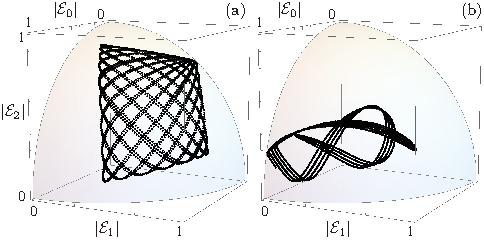
\includegraphics[width=\linewidth]{Fig3.pdf}}
\caption{(Color online) Absolute amplitude trajectories, $(\vert \mathcal{E}_{0}(z) \vert, \vert \mathcal{E}_{1}(z) \vert, \vert \mathcal{E}_{2}(z) \vert )$, for initial fields, $(\vert \mathcal{E}_{0}(0) \vert, \vert \mathcal{E}_{1}(0) \vert, \vert \mathcal{E}_{2}(0) \vert )$, impinging (a) only the zeroth (solid black), $(1,0,0)$, first (dashed blue), $(0,1,0)$, and second (dotted red), $(0,0,1)$, waveguides and (b) initial fields impinging two waveguides at a time with and without a relative phase, $(1,1,0)/ \sqrt{2}$ (solid black), $(1,i,0)/\sqrt{2}$ (dashed blue), and $(2,0,i)/\sqrt{5}$ (dotted red).}
\label{fig: Fig3}
\end{figure}




\subsection{Two identical couplings and the golden ratio}
In the case of two equal coupling parameters the unitless Hamiltonian becomes
\begin{equation}
H=\left( \begin{array}{ccc}
0 & 1 & \alpha \\
1 & 0 & \alpha \\
\alpha & \alpha & 0 \end{array} \right)	 
\end{equation}
Note that the Hamiltonian is  $\hat{Z}_2$-invariante, i.e. it is invariant under exchanging the first and the second waveguide.
This symmetry also is reflected by the eigenvalues which are  $\left\{-1, \bar{\varphi}, \varphi  \right\}$ with
\begin{eqnarray}
\bar{\varphi} &=& \frac{1}{2} \left(1-\sqrt{8 \alpha ^2+1}\right),\\
\varphi &=& \frac{1}{2} \left( 1 + \sqrt{8 \alpha ^2+1} \right).
\end{eqnarray}
It is simple to see that $\bar{\varphi} + \varphi = 1$ and that the latter eigenvalue 
becomes the golden ratio for $\alpha = \sqrt{1/2}$.
Due to the $\hat{Z}_2$-symmetry the propagator can be calculated directly using the group theory approach,
\begin{eqnarray}
\Delta(\zeta) &=& \Theta(z), \\
&=& \frac{\alpha}{\varphi - \tilde{\varphi}} \left(  e^{i \zeta \varphi }  -  e^{i \zeta \bar{\varphi} } \right), \\
\Gamma(\zeta) &=& \frac{1}{\varphi - \tilde{\varphi}} \left( \varphi e^{i \zeta \bar{\varphi} } - \bar{\varphi}  e^{i \zeta \varphi } \right), \\
\Sigma(\zeta) &=& \frac{1}{2 \left( \varphi - \tilde{\varphi} \right)} \left( \varphi e^{i \zeta \varphi } - \bar{\varphi} e^{i \zeta \bar{\varphi} } \right) - \frac{1}{2} e^{-i \zeta}, \\
\Pi(\zeta) &=& \Xi(\zeta), \\
&=& \frac{1}{2 \left( \varphi - \tilde{\varphi} \right)} \left( \varphi e^{i \zeta \varphi } - \bar{\varphi} e^{i \zeta \bar{\varphi} } \right) + \frac{1}{2} e^{-i \zeta}.
\end{eqnarray}

Obviously the three eigenvalues are stationary points of the system. 
However, this particular symmetry might allow further interesting states.
Note that the auxiliary functions $\Delta(\zeta)$ and $\Gamma(\zeta)$ depend on only two of the three eigenfrequencies, $\varphi$ and $\bar{\varphi}$. 
Furthermore, a little bit of algebra considering a initial state without any field impinging the zeroth waveguide, $\mathcal{E}_{0}=0$, reveals that propagation in the second waveguide, $\mathcal{E}_{2}(z)$, only depends on those two auxiliary functions, $\Delta(\zeta)$ and $\Gamma(\zeta)$,
\begin{equation}
\mathcal{E}_{2}(\zeta) = \Delta(\zeta)\mathcal{E}_{1}(0)
+\Gamma(\zeta)\mathcal{E}_{2}(0).
\end{equation}
Now, we can hope that choosing a proper input will cancel out one of the two 
eigenvalues that appear in the evolution of the field amplitude at the second waveguide.
That is, if the evolution only depends on a single eigenvalue, it will only change in phase and the field amplitude will remain immutable. 
Hence, lets look for such a state where no energy transfer into or out of the second waveguide occurs. 
This is fulfilled if either of the two following conditions is met,
\begin{eqnarray}
\mathcal{E}_{1}(0)= \frac{\varphi}{\alpha} \mathcal{E}_{2}(0)\quad \mathrm{or} \quad
\mathcal{E}_{1}(0)= \frac{\bar{\varphi}}{\alpha} \mathcal{E}_{2}(0).
\end{eqnarray}
Consequently we obtain two solutions for a state with stationary amplitude in the second waveguide.
Without loss of generality, we can give the propagated amplitude vector up to a normalization constant,
\begin{equation} \label{eq:StatAmp}
\vert \mathcal{E}_{x}(\zeta) \rangle =\left( \begin{array}{c}
\frac{\varphi}{\alpha} \Sigma(\zeta) + \Delta(\zeta) \\
\frac{\varphi}{\alpha} \Pi(z) + \Delta(\zeta) \\
e^{i\zeta\varphi}
\end{array} \right)	\quad x= \varphi, \bar{\varphi}.
\end{equation}

\begin{figure}[htbp]
	\centering
	\fbox{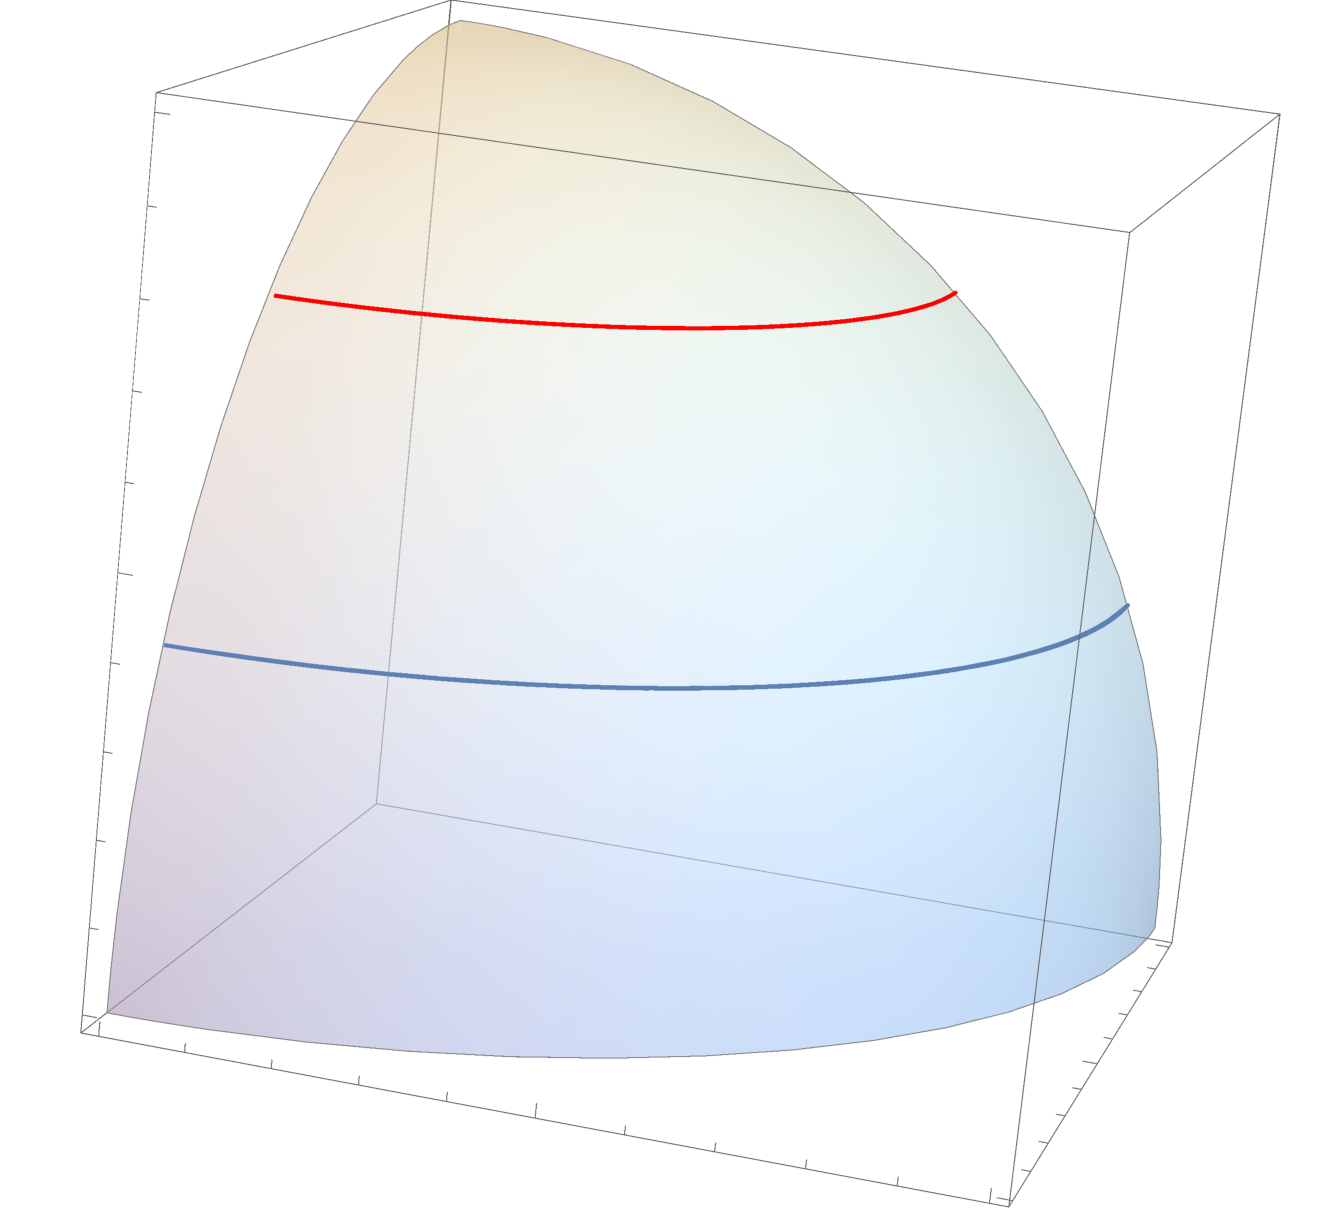
\includegraphics[height=4cm]{Fig5.pdf}}
	\caption{(Color online) Absolute amplitude trajectories, $(\vert \mathcal{E}_{0}(z) \vert, \vert \mathcal{E}_{1}(z) \vert, \vert \mathcal{E}_{2}(z) \vert )$,  for the states with stationary field amplitude in the second waveguide as obtained in Eq.(\ref{eq:StatAmp}).}
	\label{fig: Fig5}
\end{figure}



%%%%%%%%%%%%%%%%%%%%%%%
%%%% DRAFT
%//////////////////////////////////////////////%//////

\section{Classical mechanics and envelopes}
An lossless waveguide is an optical cavity, where
\textcolor{red}{something missing here ?!}\newline  
In quantum mechanics, the Hamiltonian for three coupled harmonic oscillators is given by:
\begin{eqnarray}\label{eq:qmHamiltonian}
	\hat{H}(t) = \sum_{j=0}^{2} \omega_j(t) \hat{a}^{\dagger}_j \hat{a}_{j} + \sum_{j\neq k=0}^{2} g_{jk}(t) \hat{a}^{\dagger}_j \hat{a}_k,
\end{eqnarray}
where, by analogy with equation (\ref{eq:principal}),  $\omega_j(t)$ are the time dependent free oscillator
frequencies and $g_{ij}(t)$ refer to the time dependent coupling constants. The Hamiltonian above has been studied 
elsewhere and here we will only consider two limiting cases.
The classical limit is usually associated with the coherent state solution and involves an infinite number of photons. 
The opposite end of the spectrum is marked by the single photon 
limit. At any given time only a single photon occupies the system 
and consequently the ansatz is as follows,
\begin{eqnarray}\label{eq:sglPhoton}
	\left\vert \psi(t) \right\rangle = \mathcal{E}_{0}(t) \left\vert 1, 0, 0 \right\rangle  +
	\mathcal{E}_{1}(t) \left\vert 0,1,0 \right\rangle + \mathcal{E}_{2}(t) \left\vert 0,0,1 \right\rangle,
\end{eqnarray}
with $ \sum_{j} \vert \mathcal{E}_{j}(z) \vert^2 = 1$. 
Applying the single photon state, equation (\ref{eq:sglPhoton}), to the 
quantum Hamiltonian, equation (\ref{eq:qmHamiltonian}), 
yields a differential equation set equivalent to the mode coupling theory result, Eq.(\ref{eq:ddiff}) up to substitution of backwards time by propagation distance, or, better, 
\begin{eqnarray} \label{eq:}
	i \partial_t	
	\left( \begin{array}{c} 
		\mathcal{E}_{0}(t) \\
		\mathcal{E}_{1}(t) \\
		\mathcal{E}_{2}(t)
	\end{array} \right) =
	\left( \begin{array}{ccc} 
		\omega_{0}(t)  & g_{01}(t) & g_{02}(t) \\
		g_{01}(t) & \omega_{1}(t) & g_{12}(t) \\
		g_{02}(t) & g_{12}(t) & \omega_{2}(t)
	\end{array} \right)
	\left( \begin{array}{c} 
		\mathcal{E}_{0}(t) \\
		\mathcal{E}_{1}(t) \\
		\mathcal{E}_{2}(t)
	\end{array} \right) .
\end{eqnarray}

The result above is a differential equation 
for the solution of the three coupled wave guides
with respect to the complex amplitudes of each 
wave-guide. In certain circumstances and and for 
reason that will become apparent shortly it is 
feasible to derive equations of motions 
for other sets of variables. 

We can use quadratures,
\begin{eqnarray}
	\hat{q} = \frac{1}{\sqrt{2}} \left( \hat{a}^{\dagger} + \hat{a} \right), ~ 
	\hat{p} = \frac{i}{\sqrt{2}} \left( \hat{a}^{\dagger} + \hat{a} \right),
\end{eqnarray}
and consider classical variables, where we have accounted for the change in the time propagation,
\begin{eqnarray}
	i \partial_t	
	\left( \begin{array}{c} 
		p_{0}(t) \\
		p_{1}(t) \\
		p_{2}(t)
	\end{array} \right) =
	\left( \begin{array}{ccc} 
		\omega_{0}(t)  & g_{01}(t) & g_{02}(t) \\
		g_{01}(t) & \omega_{1}(t) & g_{12}(t) \\
		g_{02}(t) & g_{12}(t) & \omega_{2}(t)
	\end{array} \right)
	\left( \begin{array}{c} 
		q_{0}(t) \\
		q_{1}(t) \\
		q_{2}(t)
	\end{array} \right) , \\
	i \partial_t	
	\left( \begin{array}{c} 
		q_{0}(t) \\
		q_{1}(t) \\
		q_{2}(t)
	\end{array} \right) = -
	\left( \begin{array}{ccc} 
		\omega_{0}(t)  & g_{01}(t) & g_{02}(t) \\
		g_{01}(t) & \omega_{1}(t) & g_{12}(t) \\
		g_{02}(t) & g_{12}(t) & \omega_{2}(t)
	\end{array} \right)
	\left( \begin{array}{c} 
		p_{0}(t) \\
		p_{1}(t) \\
		p_{2}(t)
	\end{array} \right) ,
\end{eqnarray}



\textcolor{red}{This can also be done with the idea of Euler angles for $SU(3)$ in \cite{Nelson1967p857}}

In the classical limit, the canonical pair provided by the creation and annihilation operators can be replaced by the classical canonical pair of intensity and phase, $\left\{ n_{j}, \phi_{j} \right\}$, $ \hat{a}_{j} \rightarrow \sqrt{n_{j}}e^{i \phi_{j}}$. 
This delivers a classical Hamiltonian, 
\begin{eqnarray}\label{eq:clHamiltonian}
	H(t) = \sum_{j=0}^{2} \omega_{j}(t) n_{j}  
	+ \sum_{j \neq k = 0}^{2} g_{jk} \sqrt{n_{j} n_{k}} \cos \left( \phi_{j} - \phi_{k} \right),
\end{eqnarray}
the equations of motion for the canonical pairs are 
\begin{eqnarray}
	\partial_t n_j = \frac{\partial H}{\partial \phi_j}\\
	\partial_t \phi_j = - \frac{\partial H}{\partial n_j}  
\end{eqnarray}
and these are the coupled mode equations describing the evolution of intensity and phase.

Classicam mechanics: if the three normal modes frequencies, e.g. eigenvalues of the mode-coupling matrix in Eq.(9), are commesurate then the propagated complex fields will be periodic \cite{Goldstein1980}. 

In order to visualize the dynamics of the system we will choose a (pseudo?) Poincar\'e phase-space given by the square roots of the three waveguide intensities $(\vert \mathcal{E}_{0} \vert,\vert \mathcal{E}_{1} \vert,\vert \mathcal{E}_{2} \vert )$.
Here  normal mode frequencies that are rational multiples of each other, commensurate, will translate into well-defined closed trajectories. For incommensurate normal frequencies the trajectories will be ergodic and fill a region of phase space defined by the energy of the motion \cite{Goldstein1980}.

Let us turn to the vast class of incommensurate trajectories. In many situations the exact route 
of the trajectory is not of primary importance and 
it will suffice to have gained some information on the region that will be traversed. The region 
of a given trajectory is characterised by the 
boundary which encompasses the very region. Therefore in the remainder of this section we will 
attend to finding the corresponding boundary which we also refer to as the envelope of the trajectory.   

%Note that requiring a normalized intensity in the optical system translates into $\sum_{j} n_{j} = 1$, this obviates the use of $\partial_{t} n_{2}$ and suggest taking the phase at the $j=2$ as reference as $\partial_{t} \phi_{2} = 0$. This reduces the problem by one degree of freedom to two degrees of freedom.
%
%Numerically, it makes no difference to solve Eq.(9) or use Eq.(11)-Eq.(12).
%Figure \ref{fig: Fig2} shows the squared root intensities plot for the numerical propagation of random parameter sets and initial conditions. The absolute value of the difference between the numerical propagation from the complex field or the intensity-phase picture was always below $10^{-5}$.
%We are plotting the absolute amplitudes $(\vert E_{0}(z) \vert, \vert E_{1}(z) \vert, \vert E_{2}(z) \vert )$, thus the trajectories will are on an octant of the unit sphere.

\begin{figure}[htbp]
	\centering
	\fbox{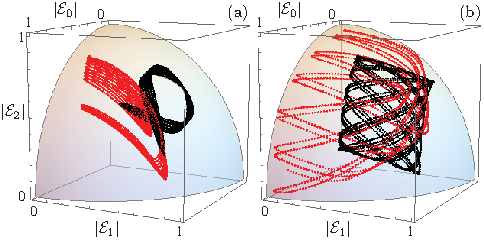
\includegraphics[width=\linewidth]{Fig2.pdf}}
	\caption{(Color online) Absolute amplitude trajectories, $(\vert E_{0}(z) \vert, \vert E_{1}(z) \vert, \vert E_{2}(z) \vert )$, for initial random fields impinging random optical trimmers with constant parameters.}
	\label{fig: Fig2}
\end{figure}

%Dealing with the problem in the intensity-phase picture does not make it easier to solve but it provides insight.
%Given a trimmer parameter set, $S(z) = \left\{ \omega_{j}(z), g_{jk}(z) \right\}$, and an initial field configuration, $\mathcal{E}(0) = \left\{ \mathcal{E}_{j}(0) \right\}$, it is possible to calculate the energy of the orbit, $H(0) = \epsilon\left(S(0), \mathcal{E(0)}\right)$. Then, it is possible to find the conditions that define the envelope of such orbit in the absolute value of the field amplitude plots via simultaneous elimination of the phase variables with $H(z) - \epsilon = 0 $ and $\partial_t \phi_j = 0$ for $j= 0,1$.


It proves viable to notice that for a given energy and a given set of parameters in most cases an infinity number of distinct trajectories prevails.
The conjunction of all these trajectories pertaining to a certain energy
span a path-connected surface.
Firstly we will be concerned with finding the outer boundary, or envelope, of the union of all trajectories pertaining to Energy 
E.
Equation (\ref{eq:clHamiltonian}) readily reveals that for given intensities 
$n_1,n_2$ and $n_3$ the energy is maximised when all three phases
are zero. Consequently the envelope is defined by all triplets
$n_1,n_2$ and $n_3$ which fulfil following condition
\begin{equation}
	H_{Bndry}(n_1,n_2,n_3) := \sum_{j=0}^{2} \omega_{j}(t) n_{j}  
	+ \sum_{j \neq k = 0}^{2} g_{jk} \sqrt{n_{j} n_{k}} = E,	
\end{equation}

Due to energy conservation, the three intensities are not 
independent and we can safely omit the third intensity in the 
following discussion, ie. 
$H_{Bndry}(n_1,n_2,n_3) \rightarrow H_{Bndry}(n_1,n_2)$.
Numerically, once a given set of initial intensities and/or
energy was chosen $H_{Bndry}(n_1,n_2) \rightarrow E$ the 
trajectory of the envelope is characterised by the following differential equation:    
\begin{eqnarray}
	\frac{\partial H_{Bndry}}{\partial n_1}\delta n_1 + 
	\frac{\partial H_{Bndry}}{\partial n_2}\delta n_2 = 0
\end{eqnarray}

Having obtained the envelope of the union of all trajectories we 
can turn to the area of a single trajectory. We recall that we 
focus our interest on parameters such that the corresponding 
trajectories are incommensurate, i.e. they fill all the area inside
a closed loop. To find the envelope of a certain trajectory, that 
is the aforementioned loop, we assume we
already have obtained 
the explicit solution for the trajectory.
Our solution is most easily expressed as 
solution to equation (\ref{eq:principal}) which is given by:
\begin{eqnarray}
	\mathcal{E}(t) = a_1 e_1 e^{i \omega_1 t} + a_2 e_2 e^{i \omega_2 t} +a_3 e_3 e^{i \omega_3 t} 
\end{eqnarray}
where $e_1,e_2$ and $e_3$ are the eigenvectors with corresponding eigenfrequencies $\omega_1, \omega_2$ and $\omega_3$. Parameters $a1, a2$ and $ a3$ are chosen in accordance with the initial values $n_1$ and $n_2$. Note 
that $n_j = \mathcal{E}_j\mathcal{E^*}_j$
\textcolor{red}{The following is a bit handwaving, we probably need to explain it better}
Incommensurate trajectories are 
characterised by broken periodicity and 
we can introduce a phase relevant parameter which controls/mimics the incommensurability: 
\begin{eqnarray}
	\mathcal{E}(t, \phi) = a_1 e_1 e^{i \omega_1 t + \phi} + a_2 e_2 e^{i \omega_2 t} +a_3 e_3 e^{i \omega_3 t} 
\end{eqnarray}
The parameter $\phi$ acts such that 
a given trajectory or more precisely a section of the trajectory is offset in a
direction perpendicular to the trajectory.
This however can not hold true at the 
boundary or envelope and hence we establish
following condition for the envelope:
\begin{eqnarray}
	\frac{ (\frac{\partial n_1}{\partial t}) }{ (\frac{\partial n_2}{\partial t}) } = \frac{( \frac{\partial n_1}{\partial \phi})}{(\frac{\partial n_2}{\partial \phi}) } 	
\end{eqnarray}
which is equal to:
\begin{eqnarray}
	D(t, \phi):=Det[\left(  \begin{array}{cc} 
		\frac{\partial n_1}{\partial t} & \frac{\partial n_2}{\partial t} \\
		\frac{\partial n_1}{\partial \phi} & \frac{\partial n_2}{\partial \phi} 
	\end{array} \right)] = 0
\end{eqnarray}
Accordingly, the envelope can be calculated numerically
from following differential equation:
\begin{eqnarray}
	\frac{\partial D(t,\phi)}{\partial t} \delta t +
	\frac{\partial D(t,\phi)}{\partial \phi} \delta \phi = 0
\end{eqnarray}

\begin{figure}[htbp]
	\centering
	\fbox{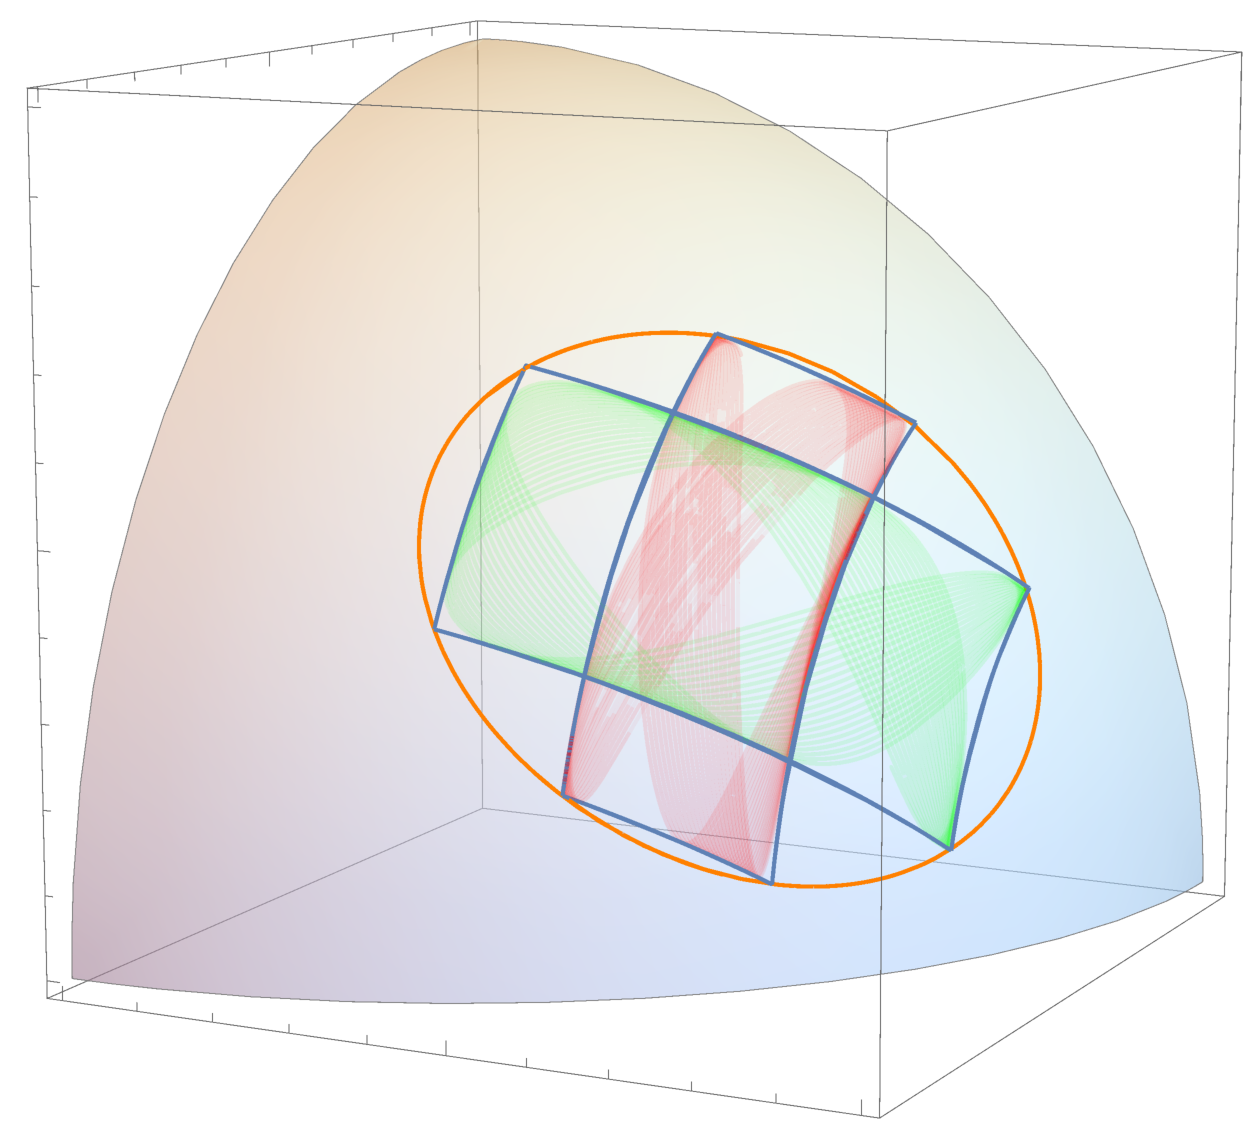
\includegraphics[height=4cm]{Fig4.pdf}}
	\caption{(Color online) Absolute amplitude trajectories, $(\vert E_{0}(z) \vert, \vert E_{1}(z) \vert, \vert E_{2}(z) \vert )$,  for two 
		distinct trajectories pertaining to 
		the energy E. The boundary 
		of all possible trajectories corresponding to energy E. The envelopes of the indivudual trajectories are are calculated according to equation ().} 
	
	\label{fig: Fig4}
\end{figure}


\section{Conclusion}
We have shown that it is possible to solve the light evolution
equations in a coupled three-core waveguide, in terms of
the Lie group generators of su(3). We focused our attention on a
reduced class of structures where the coupling constants
are constant in position......... As an
example we consider the case of equal coupling constants.
we found that the dynamics of such a system i 
governed by a linear third order differential equation and the
corresponding five auxiliary functions can be expressed in term of its solution.
we also established a connection between a waveguide cluster
with equal couplings and the well known Fourier transform, possibly opening
a path to realise quantum Fourier transformations.
furthermore we studies an isosceles waveguide triangle.
We showed that two equal couplings corresponds to
a Z2 symmetry of the Hamiltonian. We also showed 
that the symmetry allows for two interesting stated
characterised by absence of energy transfer into the 
third core.


%\section*{Funding Information}

%\textbf{Funding.} 

%\section*{Acknowledgments}

%\textbf{Acknowledgment.} 


%\section*{References}
% Bibliography
\bibliographystyle{osajnl}
\bibliography{D:/ExternalHD/Bibliography/references}


\end{document}

A secondary motivation lies in the fact that conversion from amplitude modulation to phase modulation, as well as the converse, has been shown in a $PT$-symmetric three-waveguide coupler photonic devices with $SO(2,1)$ symmetry that may provide an alternative platform to Kerr nonlinear three-waveguide couplers which have been shown to provide all-optical spatial switching \cite{Finlayson1990p2276,Stegeman1990p95,Artigas1996p53,Chen1997p287,Liu2003p2930,Khan2008p9417,Tao2011p071104} and logic gates \cite{Menezes2007p1191,Menezes2007p107,Coelho2013p731}


\section{Trimer with two identical couplings}

If we ease the general problem and allow two couplings to be equal, $g_{02}(z) = g_{12}(z) = g(z)$, it seems worthwhile trying to find a higher order differential equation for $\Delta(\zeta)$, which is the auxiliary function that connects the two sets of differential equations, Eq.(\ref{eq:set1}) and Eq.(\ref{eq:set2}).
After some algebra, it is possible to write,
\begin{equation}
\Delta^{\prime \prime}(\zeta) - \left[ i g_{01}(z) + \frac{g^{\prime}(z)}{g(z)} \right]  \Delta^{\prime}(\zeta) + 2 g^{2}(z) \Delta(\zeta) = 0,\label{eq:ddiff}
\end{equation}
with initial values,
\begin{eqnarray}
\Delta(0) & = & 0 , \\
\Delta^{\prime}(0) &=& i g(0). 
\end{eqnarray}
In this case, the remaining auxiliary functions are given by the following expressions,

For example, the case of a constant coupling, $g_{01}$, and two sinusoidal coupling functions, 
\begin{eqnarray}
g(z) = g_{01} \left[ 1 + \alpha \sin \left( k z \right) \right], \quad \vert \alpha \vert < 1,
\end{eqnarray}

In operator form the propagator yields
\begin{eqnarray}
U(\zeta)=\Sigma(\zeta)\;(I_{+}+I_{-})
+\Delta(\zeta)\;(U_{+}+U_{-}+V_{+}+V_{-})
\nonumber\\
+\frac{2}{3}\left[ \Pi(\zeta) - \Gamma(\zeta) \right]\;(U_{0}+V_{0})  
+\frac{1}{3}\left[ \Gamma(\zeta) + 2 \Pi(\zeta) \right]\;\mathbbm{1}.
\end{eqnarray}
>>>>>>> 0aa4f510b5d14d04eb2b582fe0ae7fa29973b3f7
